% Options for packages loaded elsewhere
\PassOptionsToPackage{unicode}{hyperref}
\PassOptionsToPackage{hyphens}{url}
%
\documentclass[
  12pt,
]{article}
\usepackage{amsmath,amssymb}
\usepackage{lmodern}
\usepackage{ifxetex,ifluatex}
\ifnum 0\ifxetex 1\fi\ifluatex 1\fi=0 % if pdftex
  \usepackage[T1]{fontenc}
  \usepackage[utf8]{inputenc}
  \usepackage{textcomp} % provide euro and other symbols
\else % if luatex or xetex
  \usepackage{unicode-math}
  \defaultfontfeatures{Scale=MatchLowercase}
  \defaultfontfeatures[\rmfamily]{Ligatures=TeX,Scale=1}
\fi
% Use upquote if available, for straight quotes in verbatim environments
\IfFileExists{upquote.sty}{\usepackage{upquote}}{}
\IfFileExists{microtype.sty}{% use microtype if available
  \usepackage[]{microtype}
  \UseMicrotypeSet[protrusion]{basicmath} % disable protrusion for tt fonts
}{}
\usepackage{xcolor}
\IfFileExists{xurl.sty}{\usepackage{xurl}}{} % add URL line breaks if available
\IfFileExists{bookmark.sty}{\usepackage{bookmark}}{\usepackage{hyperref}}
\hypersetup{
  pdftitle={hw1},
  pdfauthor={Liming Ning},
  hidelinks,
  pdfcreator={LaTeX via pandoc}}
\urlstyle{same} % disable monospaced font for URLs
\usepackage[margin=1in]{geometry}
\usepackage{color}
\usepackage{fancyvrb}
\newcommand{\VerbBar}{|}
\newcommand{\VERB}{\Verb[commandchars=\\\{\}]}
\DefineVerbatimEnvironment{Highlighting}{Verbatim}{commandchars=\\\{\}}
% Add ',fontsize=\small' for more characters per line
\usepackage{framed}
\definecolor{shadecolor}{RGB}{248,248,248}
\newenvironment{Shaded}{\begin{snugshade}}{\end{snugshade}}
\newcommand{\AlertTok}[1]{\textcolor[rgb]{0.94,0.16,0.16}{#1}}
\newcommand{\AnnotationTok}[1]{\textcolor[rgb]{0.56,0.35,0.01}{\textbf{\textit{#1}}}}
\newcommand{\AttributeTok}[1]{\textcolor[rgb]{0.77,0.63,0.00}{#1}}
\newcommand{\BaseNTok}[1]{\textcolor[rgb]{0.00,0.00,0.81}{#1}}
\newcommand{\BuiltInTok}[1]{#1}
\newcommand{\CharTok}[1]{\textcolor[rgb]{0.31,0.60,0.02}{#1}}
\newcommand{\CommentTok}[1]{\textcolor[rgb]{0.56,0.35,0.01}{\textit{#1}}}
\newcommand{\CommentVarTok}[1]{\textcolor[rgb]{0.56,0.35,0.01}{\textbf{\textit{#1}}}}
\newcommand{\ConstantTok}[1]{\textcolor[rgb]{0.00,0.00,0.00}{#1}}
\newcommand{\ControlFlowTok}[1]{\textcolor[rgb]{0.13,0.29,0.53}{\textbf{#1}}}
\newcommand{\DataTypeTok}[1]{\textcolor[rgb]{0.13,0.29,0.53}{#1}}
\newcommand{\DecValTok}[1]{\textcolor[rgb]{0.00,0.00,0.81}{#1}}
\newcommand{\DocumentationTok}[1]{\textcolor[rgb]{0.56,0.35,0.01}{\textbf{\textit{#1}}}}
\newcommand{\ErrorTok}[1]{\textcolor[rgb]{0.64,0.00,0.00}{\textbf{#1}}}
\newcommand{\ExtensionTok}[1]{#1}
\newcommand{\FloatTok}[1]{\textcolor[rgb]{0.00,0.00,0.81}{#1}}
\newcommand{\FunctionTok}[1]{\textcolor[rgb]{0.00,0.00,0.00}{#1}}
\newcommand{\ImportTok}[1]{#1}
\newcommand{\InformationTok}[1]{\textcolor[rgb]{0.56,0.35,0.01}{\textbf{\textit{#1}}}}
\newcommand{\KeywordTok}[1]{\textcolor[rgb]{0.13,0.29,0.53}{\textbf{#1}}}
\newcommand{\NormalTok}[1]{#1}
\newcommand{\OperatorTok}[1]{\textcolor[rgb]{0.81,0.36,0.00}{\textbf{#1}}}
\newcommand{\OtherTok}[1]{\textcolor[rgb]{0.56,0.35,0.01}{#1}}
\newcommand{\PreprocessorTok}[1]{\textcolor[rgb]{0.56,0.35,0.01}{\textit{#1}}}
\newcommand{\RegionMarkerTok}[1]{#1}
\newcommand{\SpecialCharTok}[1]{\textcolor[rgb]{0.00,0.00,0.00}{#1}}
\newcommand{\SpecialStringTok}[1]{\textcolor[rgb]{0.31,0.60,0.02}{#1}}
\newcommand{\StringTok}[1]{\textcolor[rgb]{0.31,0.60,0.02}{#1}}
\newcommand{\VariableTok}[1]{\textcolor[rgb]{0.00,0.00,0.00}{#1}}
\newcommand{\VerbatimStringTok}[1]{\textcolor[rgb]{0.31,0.60,0.02}{#1}}
\newcommand{\WarningTok}[1]{\textcolor[rgb]{0.56,0.35,0.01}{\textbf{\textit{#1}}}}
\usepackage{graphicx}
\makeatletter
\def\maxwidth{\ifdim\Gin@nat@width>\linewidth\linewidth\else\Gin@nat@width\fi}
\def\maxheight{\ifdim\Gin@nat@height>\textheight\textheight\else\Gin@nat@height\fi}
\makeatother
% Scale images if necessary, so that they will not overflow the page
% margins by default, and it is still possible to overwrite the defaults
% using explicit options in \includegraphics[width, height, ...]{}
\setkeys{Gin}{width=\maxwidth,height=\maxheight,keepaspectratio}
% Set default figure placement to htbp
\makeatletter
\def\fps@figure{htbp}
\makeatother
\setlength{\emergencystretch}{3em} % prevent overfull lines
\providecommand{\tightlist}{%
  \setlength{\itemsep}{0pt}\setlength{\parskip}{0pt}}
\setcounter{secnumdepth}{-\maxdimen} % remove section numbering
\usepackage{booktabs}
\usepackage{longtable}
\usepackage{array}
\usepackage{multirow}
\usepackage{wrapfig}
\usepackage{float}
\usepackage{colortbl}
\usepackage{pdflscape}
\usepackage{tabu}
\usepackage{threeparttable}
\usepackage{threeparttablex}
\usepackage[normalem]{ulem}
\usepackage{makecell}
\usepackage{xcolor}
\ifluatex
  \usepackage{selnolig}  % disable illegal ligatures
\fi

\title{hw1}
\author{Liming Ning}
\date{2022/1/16}

\begin{document}
\maketitle

{
\setcounter{tocdepth}{2}
\tableofcontents
}
\hypertarget{case-study-1-audience-size}{%
\section{Case Study 1: Audience Size}\label{case-study-1-audience-size}}

\hypertarget{data-preparation}{%
\subsection{Data Preparation}\label{data-preparation}}

\hypertarget{cleaning}{%
\subsubsection{cleaning}\label{cleaning}}

\begin{Shaded}
\begin{Highlighting}[]
\CommentTok{\# selection}
\NormalTok{talkdata }\OtherTok{=} \FunctionTok{fread}\NormalTok{(}\StringTok{"data/Survey\_results\_final.csv"}\NormalTok{, }\AttributeTok{encoding =} \StringTok{"UTF{-}8"}\NormalTok{)}
\NormalTok{talkdata.selected }\OtherTok{=} 
\NormalTok{  talkdata[,.(}\AttributeTok{age =}\NormalTok{ Answer.Age, }\CommentTok{\# Note: some answers in Age are not numerics. Therefore, typeof Answer.Age is character.}
              \AttributeTok{gender =}\NormalTok{ Answer.Gender, }
              \AttributeTok{education =}\NormalTok{ Answer.Education, }
              \AttributeTok{income =}\NormalTok{ Answer.HouseHoldIncome,}
              \AttributeTok{sirius =} \StringTok{\textasciigrave{}}\AttributeTok{Answer.Sirius Radio}\StringTok{\textasciigrave{}}\NormalTok{, }
              \AttributeTok{wharton =} \StringTok{\textasciigrave{}}\AttributeTok{Answer.Wharton Radio}\StringTok{\textasciigrave{}}\NormalTok{, }
              \AttributeTok{worktime =}\NormalTok{ WorkTimeInSeconds)]}
\NormalTok{talkdata}\SpecialCharTok{$}\NormalTok{Reward[}\DecValTok{1}\SpecialCharTok{:}\DecValTok{10}\NormalTok{] }\CommentTok{\# question: 5 cents or 10 cents?}
\end{Highlighting}
\end{Shaded}

\begin{verbatim}
##  [1] "$0.05" "$0.05" "$0.05" "$0.05" "$0.05" "$0.05" "$0.05" "$0.05" "$0.05"
## [10] "$0.05"
\end{verbatim}

\begin{Shaded}
\begin{Highlighting}[]
\CommentTok{\# detect suspect observations}
\DocumentationTok{\#\# age}
\NormalTok{talkdata.selected[}\SpecialCharTok{!}\NormalTok{age }\SpecialCharTok{\%in\%} \DecValTok{10}\SpecialCharTok{:}\DecValTok{100}\NormalTok{] }\CommentTok{\# automatic type coersion when matching}
\end{Highlighting}
\end{Shaded}

\begin{verbatim}
##              age gender                                       education
## 1:                 Male                                      select one
## 2:           223   Male            High school graduate (or equivalent)
## 3:        female Female Some college, no diploma; or Associate’s degree
## 4: Eighteen (18)   Male            High school graduate (or equivalent)
## 5:             4   Male        Bachelor’s degree or other 4-year degree
## 6:           27`   Male Some college, no diploma; or Associate’s degree
##               income sirius wharton worktime
## 1:                                         5
## 2: $30,000 - $50,000     No      No       11
## 3:    Above $150,000    Yes      No       21
## 4: $30,000 - $50,000    Yes      No       29
## 5: $50,000 - $75,000    Yes      No       22
## 6: Less than $15,000     No      No       20
\end{verbatim}

\begin{Shaded}
\begin{Highlighting}[]
\NormalTok{talkdata.selected[age }\SpecialCharTok{==} \StringTok{"Eighteen (18)"}\NormalTok{, age }\SpecialCharTok{:}\ErrorTok{=} \StringTok{"18"}\NormalTok{] }\CommentTok{\# imputation}
\NormalTok{talkdata.selected[age }\SpecialCharTok{==} \StringTok{"27\textasciigrave{}"}\NormalTok{, age }\SpecialCharTok{:}\ErrorTok{=} \StringTok{"27"}\NormalTok{] }\CommentTok{\# imputation}
\NormalTok{talkdata.selected }\OtherTok{=}\NormalTok{ talkdata.selected[age }\SpecialCharTok{\%in\%} \DecValTok{10}\SpecialCharTok{:}\DecValTok{100}\NormalTok{] }\CommentTok{\# delete NAs}
\NormalTok{talkdata.selected[,age }\SpecialCharTok{:}\ErrorTok{=} \FunctionTok{as.numeric}\NormalTok{(age)]}

\DocumentationTok{\#\# gender}
\FunctionTok{unique}\NormalTok{(talkdata.selected}\SpecialCharTok{$}\NormalTok{gender)}
\end{Highlighting}
\end{Shaded}

\begin{verbatim}
## [1] "Female" "Male"   ""
\end{verbatim}

\begin{Shaded}
\begin{Highlighting}[]
\NormalTok{talkdata.selected[}\SpecialCharTok{!}\NormalTok{gender }\SpecialCharTok{\%in\%} \FunctionTok{c}\NormalTok{(}\StringTok{"Male"}\NormalTok{,}\StringTok{"Female"}\NormalTok{)]}
\end{Highlighting}
\end{Shaded}

\begin{verbatim}
##    age gender                                       education            income
## 1:  47                        Graduate or professional degree $30,000 - $50,000
## 2:  47                        Graduate or professional degree $50,000 - $75,000
## 3:  29        Some college, no diploma; or Associate’s degree $15,000 - $30,000
## 4:  31                        Graduate or professional degree $30,000 - $50,000
## 5:  25        Some college, no diploma; or Associate’s degree Less than $15,000
## 6:  67        Some college, no diploma; or Associate’s degree $50,000 - $75,000
##    sirius wharton worktime
## 1:    Yes      No       54
## 2:    Yes      No       15
## 3:    Yes      No       19
## 4:     No      No       15
## 5:    Yes      No       19
## 6:     No      No       32
\end{verbatim}

\begin{Shaded}
\begin{Highlighting}[]
\NormalTok{talkdata.selected }\OtherTok{=}\NormalTok{ talkdata.selected[gender }\SpecialCharTok{!=} \StringTok{""}\NormalTok{] }\CommentTok{\# delete blanks}

\DocumentationTok{\#\# education}
\FunctionTok{unique}\NormalTok{(talkdata.selected}\SpecialCharTok{$}\NormalTok{education)}
\end{Highlighting}
\end{Shaded}

\begin{verbatim}
## [1] "Some college, no diploma; or Associate’s degree"
## [2] "Graduate or professional degree"                
## [3] "Bachelor’s degree or other 4-year degree"       
## [4] "High school graduate (or equivalent)"           
## [5] "Less than 12 years; no high school diploma"     
## [6] "select one"                                     
## [7] "Other"
\end{verbatim}

\begin{Shaded}
\begin{Highlighting}[]
\NormalTok{talkdata.selected }\OtherTok{=}\NormalTok{ talkdata.selected[}\SpecialCharTok{!}\NormalTok{education }\SpecialCharTok{\%in\%} \FunctionTok{c}\NormalTok{(}\StringTok{"Other"}\NormalTok{,}\StringTok{"select one"}\NormalTok{)] }\CommentTok{\# delete because they are meaningless}

\DocumentationTok{\#\# income}
\FunctionTok{unique}\NormalTok{(talkdata.selected}\SpecialCharTok{$}\NormalTok{income)}
\end{Highlighting}
\end{Shaded}

\begin{verbatim}
## [1] "$30,000 - $50,000"  "$15,000 - $30,000"  "$50,000 - $75,000" 
## [4] "Above $150,000"     "Less than $15,000"  "$75,000 - $150,000"
## [7] ""
\end{verbatim}

\begin{Shaded}
\begin{Highlighting}[]
\NormalTok{talkdata.selected }\OtherTok{=}\NormalTok{ talkdata.selected[income }\SpecialCharTok{!=} \StringTok{""}\NormalTok{] }\CommentTok{\# delete blanks}

\DocumentationTok{\#\# sirius}
\FunctionTok{unique}\NormalTok{(talkdata.selected}\SpecialCharTok{$}\NormalTok{sirius)}
\end{Highlighting}
\end{Shaded}

\begin{verbatim}
## [1] "No"  "Yes" ""
\end{verbatim}

\begin{Shaded}
\begin{Highlighting}[]
\NormalTok{talkdata.selected }\OtherTok{=}\NormalTok{ talkdata.selected[sirius }\SpecialCharTok{!=} \StringTok{""}\NormalTok{] }\CommentTok{\# delete blanks}

\DocumentationTok{\#\# wharton}
\FunctionTok{unique}\NormalTok{(talkdata.selected}\SpecialCharTok{$}\NormalTok{wharton)}
\end{Highlighting}
\end{Shaded}

\begin{verbatim}
## [1] "No"  "Yes" ""
\end{verbatim}

\begin{Shaded}
\begin{Highlighting}[]
\NormalTok{talkdata.selected }\OtherTok{=}\NormalTok{ talkdata.selected[wharton }\SpecialCharTok{!=} \StringTok{""}\NormalTok{] }\CommentTok{\# delete blanks}
\NormalTok{talkdata.selected[sirius }\SpecialCharTok{==} \StringTok{"No"} \SpecialCharTok{\&}\NormalTok{ wharton }\SpecialCharTok{==} \StringTok{"Yes"}\NormalTok{] }\CommentTok{\# These two are weird. Delete}
\end{Highlighting}
\end{Shaded}

\begin{verbatim}
##    age gender                            education            income sirius
## 1:  25   Male High school graduate (or equivalent) $15,000 - $30,000     No
## 2:  26   Male High school graduate (or equivalent) $15,000 - $30,000     No
##    wharton worktime
## 1:     Yes       20
## 2:     Yes       25
\end{verbatim}

\begin{Shaded}
\begin{Highlighting}[]
\NormalTok{talkdata.selected }\OtherTok{=}\NormalTok{ talkdata.selected[}\SpecialCharTok{!}\NormalTok{(sirius }\SpecialCharTok{==} \StringTok{"No"} \SpecialCharTok{\&}\NormalTok{ wharton }\SpecialCharTok{==} \StringTok{"Yes"}\NormalTok{)]}

\FunctionTok{fwrite}\NormalTok{(talkdata.selected,}\StringTok{"data/talkdata\_cleaned.csv"}\NormalTok{,}\AttributeTok{row.names =}\NormalTok{ F)}
\FunctionTok{rm}\NormalTok{(}\AttributeTok{list =} \FunctionTok{ls}\NormalTok{())}
\DocumentationTok{\#\# worktime: automatically recorded.}
\CommentTok{\# possible improvements: use dplyr. get summary stats in one go and make imputation/dropping them.}
\CommentTok{\# alternatives: do not delete some obs which seems to be valid expect for some missings/errors while we\textquotesingle{}re not running a regression with the covariates}
\end{Highlighting}
\end{Shaded}

\hypertarget{summary-stats}{%
\subsubsection{summary stats}\label{summary-stats}}

\begin{Shaded}
\begin{Highlighting}[]
\CommentTok{\# age and worktime, integer}
\NormalTok{talkdata.selected }\OtherTok{=} \FunctionTok{fread}\NormalTok{(}\StringTok{"data/talkdata\_cleaned.csv"}\NormalTok{,}\AttributeTok{encoding =} \StringTok{"UTF{-}8"}\NormalTok{)}
\NormalTok{age.stat }\OtherTok{=}\NormalTok{ talkdata.selected }\SpecialCharTok{\%\textgreater{}\%} 
  \FunctionTok{summarise}\NormalTok{(}\AttributeTok{mean =} \FunctionTok{mean}\NormalTok{(age),}\AttributeTok{min =} \FunctionTok{min}\NormalTok{(age),}\AttributeTok{median =} \FunctionTok{median}\NormalTok{(age),}\AttributeTok{max =} \FunctionTok{max}\NormalTok{(age),}\StringTok{"std. dev."} \OtherTok{=} \FunctionTok{sd}\NormalTok{(age))}
\NormalTok{worktime.stat }\OtherTok{=}\NormalTok{ talkdata.selected }\SpecialCharTok{\%\textgreater{}\%} 
  \FunctionTok{summarise}\NormalTok{(}\AttributeTok{mean =} \FunctionTok{mean}\NormalTok{(worktime),}\AttributeTok{min =} \FunctionTok{min}\NormalTok{(age),}\AttributeTok{median =} \FunctionTok{median}\NormalTok{(worktime),}\AttributeTok{max =} \FunctionTok{max}\NormalTok{(age), }\StringTok{"std. dev."} \OtherTok{=} \FunctionTok{sd}\NormalTok{(worktime))}
\NormalTok{cont.var.stat }\OtherTok{=} \FunctionTok{rbind}\NormalTok{(age.stat,worktime.stat)}
\FunctionTok{rownames}\NormalTok{(cont.var.stat) }\OtherTok{=} \FunctionTok{c}\NormalTok{(}\StringTok{"age"}\NormalTok{,}\StringTok{"worktime"}\NormalTok{)}
\NormalTok{talkdata.size }\OtherTok{=} \FunctionTok{nrow}\NormalTok{(talkdata.selected)}
\FunctionTok{kbl}\NormalTok{(cont.var.stat, }\AttributeTok{caption =} \StringTok{"Summary Statistics for Non{-}categorical Variables"}\NormalTok{, }\AttributeTok{digits =} \DecValTok{2}\NormalTok{, }\AttributeTok{booktabs =}\NormalTok{ T,}
    \AttributeTok{align =} \StringTok{"lccccc"}\NormalTok{) }\SpecialCharTok{\%\textgreater{}\%}
  \FunctionTok{kable\_styling}\NormalTok{(}\AttributeTok{latex\_options =} \FunctionTok{c}\NormalTok{(}\StringTok{"HOLD\_position"}\NormalTok{))}\SpecialCharTok{\%\textgreater{}\%}
   \FunctionTok{footnote}\NormalTok{(}\AttributeTok{general =} \FunctionTok{paste}\NormalTok{(}\StringTok{"The table reports the summary statistics for non{-}categorical variables in the talkshow data. The valid sample size is "}\NormalTok{,talkdata.size,}\StringTok{"."}\NormalTok{,}\AttributeTok{sep =} \StringTok{""}\NormalTok{),}
            \AttributeTok{threeparttable =}\NormalTok{ T)}
\end{Highlighting}
\end{Shaded}

\begin{table}[H]

\caption{\label{tab:unnamed-chunk-2}Summary Statistics for Non-categorical Variables}
\centering
\begin{threeparttable}
\begin{tabular}[t]{llcccc}
\toprule
  & mean & min & median & max & std. dev.\\
\midrule
age & 30.29 & 18 & 28 & 76 & 9.84\\
worktime & 22.49 & 18 & 21 & 76 & 9.30\\
\bottomrule
\end{tabular}
\begin{tablenotes}
\item \textit{Note: } 
\item The table reports the summary statistics for non-categorical variables in the talkshow data. The valid sample size is 1723.
\end{tablenotes}
\end{threeparttable}
\end{table}

\begin{Shaded}
\begin{Highlighting}[]
\NormalTok{age.hist }\OtherTok{=} \FunctionTok{ggplot}\NormalTok{(talkdata.selected,}\FunctionTok{aes}\NormalTok{(}\AttributeTok{x=}\NormalTok{age))}\SpecialCharTok{+}
  \FunctionTok{geom\_histogram}\NormalTok{()}\SpecialCharTok{+}
  \FunctionTok{theme\_bw}\NormalTok{()}\SpecialCharTok{+}
  \FunctionTok{labs}\NormalTok{(}\AttributeTok{title =} \StringTok{"Histogram for Ages"}\NormalTok{)}
\NormalTok{worktime.hist }\OtherTok{=} \FunctionTok{ggplot}\NormalTok{(talkdata.selected,}\FunctionTok{aes}\NormalTok{(}\AttributeTok{x=}\NormalTok{worktime))}\SpecialCharTok{+}
  \FunctionTok{geom\_histogram}\NormalTok{()}\SpecialCharTok{+}
  \FunctionTok{theme\_bw}\NormalTok{()}\SpecialCharTok{+}
  \FunctionTok{labs}\NormalTok{(}\AttributeTok{title =} \StringTok{"Histogram for Worktime"}\NormalTok{)}
\FunctionTok{plot\_grid}\NormalTok{(age.hist,worktime.hist,}\AttributeTok{nrow =} \DecValTok{1}\NormalTok{) }\CommentTok{\# right{-}skewed}
\end{Highlighting}
\end{Shaded}

\begin{verbatim}
## `stat_bin()` using `bins = 30`. Pick better value with `binwidth`.
## `stat_bin()` using `bins = 30`. Pick better value with `binwidth`.
\end{verbatim}

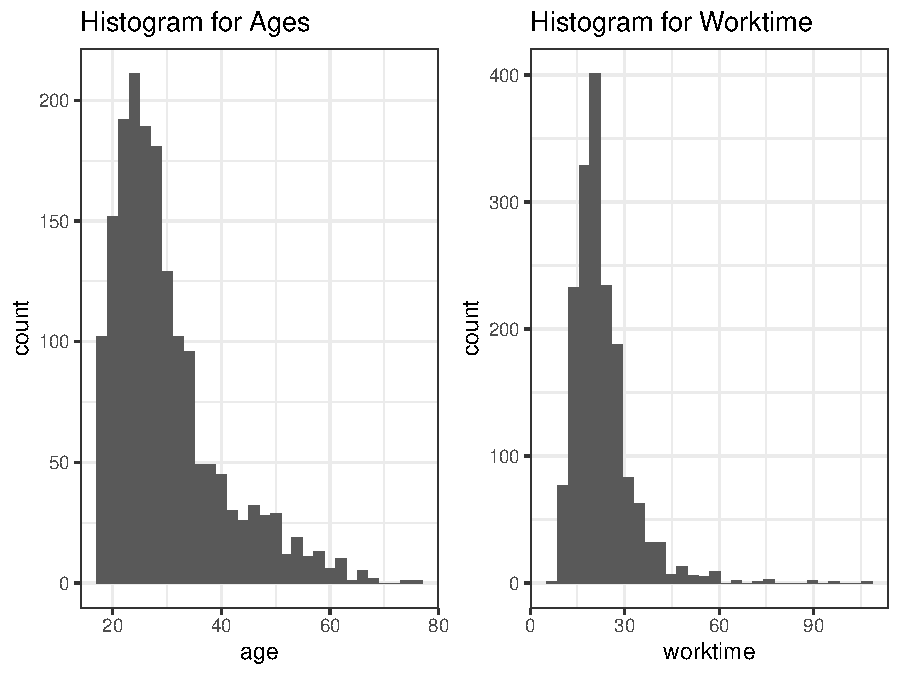
\includegraphics{hw1_sol_files/figure-latex/unnamed-chunk-2-1.pdf}

\begin{Shaded}
\begin{Highlighting}[]
\CommentTok{\# categorical variables}
\DocumentationTok{\#\# mapping}
\NormalTok{keywords.edu }\OtherTok{=} \FunctionTok{data.table}\NormalTok{(}\AttributeTok{education =} \FunctionTok{unique}\NormalTok{(talkdata.selected}\SpecialCharTok{$}\NormalTok{education))}
\NormalTok{keywords.edu[,order }\SpecialCharTok{:}\ErrorTok{=} \FunctionTok{c}\NormalTok{(}\DecValTok{3}\NormalTok{,}\DecValTok{5}\NormalTok{,}\DecValTok{4}\NormalTok{,}\DecValTok{2}\NormalTok{,}\DecValTok{1}\NormalTok{)]}
\NormalTok{keywords.edu }\OtherTok{=}\NormalTok{ keywords.edu[}\FunctionTok{order}\NormalTok{(order)]}
\ControlFlowTok{for}\NormalTok{ (i }\ControlFlowTok{in} \DecValTok{1}\SpecialCharTok{:}\FunctionTok{nrow}\NormalTok{(keywords.edu)) \{}
\NormalTok{  talkdata.selected[education}\SpecialCharTok{==}\NormalTok{keywords.edu}\SpecialCharTok{$}\NormalTok{education[i],education}\SpecialCharTok{:}\ErrorTok{=}\NormalTok{keywords.edu}\SpecialCharTok{$}\NormalTok{order[i]]}
\NormalTok{\} }\CommentTok{\# for education}

\NormalTok{keywords.income }\OtherTok{=} \FunctionTok{data.table}\NormalTok{(}\AttributeTok{income =} \FunctionTok{unique}\NormalTok{(talkdata.selected}\SpecialCharTok{$}\NormalTok{income))}
\NormalTok{keywords.income[,order }\SpecialCharTok{:}\ErrorTok{=} \FunctionTok{c}\NormalTok{(}\DecValTok{3}\NormalTok{,}\DecValTok{2}\NormalTok{,}\DecValTok{4}\NormalTok{,}\DecValTok{6}\NormalTok{,}\DecValTok{1}\NormalTok{,}\DecValTok{5}\NormalTok{)]}
\NormalTok{keywords.income }\OtherTok{=}\NormalTok{ keywords.income[}\FunctionTok{order}\NormalTok{(order)]}
\ControlFlowTok{for}\NormalTok{ (i }\ControlFlowTok{in} \DecValTok{1}\SpecialCharTok{:}\FunctionTok{nrow}\NormalTok{(keywords.income)) \{}
\NormalTok{  talkdata.selected[income}\SpecialCharTok{==}\NormalTok{keywords.income}\SpecialCharTok{$}\NormalTok{income[i],income}\SpecialCharTok{:}\ErrorTok{=}\NormalTok{keywords.income}\SpecialCharTok{$}\NormalTok{order[i]]}
\NormalTok{\} }\CommentTok{\# for income}

\DocumentationTok{\#\# plots}
\NormalTok{get.bar }\OtherTok{=} \ControlFlowTok{function}\NormalTok{(data,varname,}\AttributeTok{x.label =}\NormalTok{ varname,}\AttributeTok{y.label =} \StringTok{"count"}\NormalTok{,...)\{}

  \FunctionTok{ggplot}\NormalTok{(data,}\FunctionTok{aes}\NormalTok{(}\AttributeTok{x=}\FunctionTok{eval}\NormalTok{(}\FunctionTok{parse}\NormalTok{(}\AttributeTok{text =}\NormalTok{ varname))))}\SpecialCharTok{+}
    \FunctionTok{geom\_bar}\NormalTok{(...)}\SpecialCharTok{+}
    \FunctionTok{xlab}\NormalTok{(x.label)}\SpecialCharTok{+}
    \FunctionTok{theme\_bw}\NormalTok{()}\SpecialCharTok{+}
    \FunctionTok{labs}\NormalTok{(}\AttributeTok{title =} \FunctionTok{paste}\NormalTok{(}\StringTok{"Barplot of "}\NormalTok{,varname,}\AttributeTok{sep =} \StringTok{""}\NormalTok{))}
\NormalTok{\}}

\NormalTok{bar.list }\OtherTok{=} \FunctionTok{list}\NormalTok{()}
\NormalTok{key.catevar }\OtherTok{=} \FunctionTok{c}\NormalTok{(}\StringTok{"gender"}\NormalTok{,}\StringTok{"education"}\NormalTok{,}\StringTok{"income"}\NormalTok{,}\StringTok{"sirius"}\NormalTok{,}\StringTok{"wharton"}\NormalTok{)}
\ControlFlowTok{for}\NormalTok{ (i }\ControlFlowTok{in} \DecValTok{1}\SpecialCharTok{:}\FunctionTok{length}\NormalTok{(key.catevar)) \{}
\NormalTok{  bar.list[[i]] }\OtherTok{=} \FunctionTok{get.bar}\NormalTok{(talkdata.selected,key.catevar[i])}
\NormalTok{\}}
\FunctionTok{plot\_grid}\NormalTok{(}\AttributeTok{plotlist =}\NormalTok{ bar.list,}\AttributeTok{nrow =} \DecValTok{2}\NormalTok{)}
\end{Highlighting}
\end{Shaded}

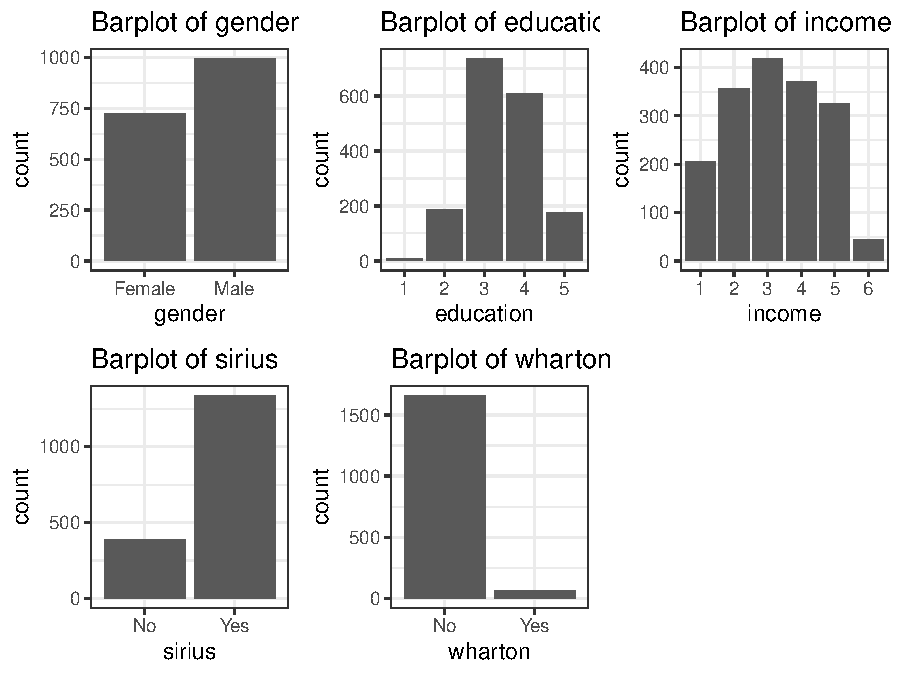
\includegraphics{hw1_sol_files/figure-latex/unnamed-chunk-2-2.pdf}

\textbf{Notes}: We map the education and income levels into integers for
better exhibition. For education, 1 means
\textit {less than 12 years; no high school diploma}, 2 means
\textit{   
High school graduate (or equivalent)}, 3 means
\textit{Some college, no diploma; or Associate’s degree}, 4 means
\textit{Bachelor’s degree or other 4-year degree}, 5 means \textit{    
Graduate or professional degree}. For income, 1 means
\textit{Less than \$15,000}, 2 means \textit{ 
\$15,000 - \$30,000}, 3 means \textit{\$30,000 - \$50,000}, 4 means
\textit{    
\$50,000 - \$75,000}, 5 means \textit{
\$75,000 - \$150,000}, 6 means \textit{Above \$150,000}.

\hypertarget{sample-properties}{%
\subsection{Sample Properties}\label{sample-properties}}

\begin{Shaded}
\begin{Highlighting}[]
\CommentTok{\# what\textquotesingle{}s the dist? to be found}
\CommentTok{\# multivariate t{-}stats}
\end{Highlighting}
\end{Shaded}

\hypertarget{final-estimates}{%
\subsection{Final Estimates}\label{final-estimates}}

\begin{Shaded}
\begin{Highlighting}[]
\NormalTok{p }\OtherTok{=} \FunctionTok{sum}\NormalTok{(talkdata.selected}\SpecialCharTok{$}\NormalTok{wharton}\SpecialCharTok{==}\StringTok{"Yes"}\NormalTok{)}\SpecialCharTok{/}\FunctionTok{sum}\NormalTok{(talkdata.selected}\SpecialCharTok{$}\NormalTok{sirius}\SpecialCharTok{==}\StringTok{"Yes"}\NormalTok{)}
\NormalTok{sigma }\OtherTok{=} \FunctionTok{sqrt}\NormalTok{(p}\SpecialCharTok{*}\NormalTok{(}\DecValTok{1}\SpecialCharTok{{-}}\NormalTok{p)}\SpecialCharTok{/}\FunctionTok{sum}\NormalTok{(talkdata.selected}\SpecialCharTok{$}\NormalTok{sirius}\SpecialCharTok{==}\StringTok{"Yes"}\NormalTok{)) }\CommentTok{\# use clt}
\FunctionTok{paste}\NormalTok{(}\StringTok{"95\% CI: ["}\NormalTok{,}\FunctionTok{round}\NormalTok{(p}\FloatTok{{-}1.96}\SpecialCharTok{*}\NormalTok{sigma,}\AttributeTok{digits =} \DecValTok{3}\NormalTok{),}\StringTok{", "}\NormalTok{,}\FunctionTok{round}\NormalTok{(p}\FloatTok{+1.96}\SpecialCharTok{*}\NormalTok{sigma,}\AttributeTok{digits =} \DecValTok{3}\NormalTok{),}\StringTok{"]."}\NormalTok{,}\AttributeTok{sep =} \StringTok{""}\NormalTok{)}
\end{Highlighting}
\end{Shaded}

\begin{verbatim}
## [1] "95% CI: [0.038, 0.062]."
\end{verbatim}

\hypertarget{new-task}{%
\subsection{New Task}\label{new-task}}

\begin{Shaded}
\begin{Highlighting}[]
\CommentTok{\# why not contact Sirius for data?}
\end{Highlighting}
\end{Shaded}

\begin{Shaded}
\begin{Highlighting}[]
\FunctionTok{rm}\NormalTok{(}\AttributeTok{list =} \FunctionTok{ls}\NormalTok{())}
\end{Highlighting}
\end{Shaded}

\hypertarget{case-study-2-women-in-science}{%
\section{Case Study 2: Women in
Science}\label{case-study-2-women-in-science}}

\hypertarget{data-preparation-1}{%
\subsection{Data Preparation}\label{data-preparation-1}}

\begin{Shaded}
\begin{Highlighting}[]
\NormalTok{degreedata }\OtherTok{=} \FunctionTok{read\_excel}\NormalTok{(}\StringTok{"Data/WomenData\_06\_16.xlsx"}\NormalTok{)}
\NormalTok{degreedata }\OtherTok{=} \FunctionTok{data.table}\NormalTok{(degreedata)}
\FunctionTok{setnames}\NormalTok{(degreedata,}\DecValTok{1}\SpecialCharTok{:}\DecValTok{5}\NormalTok{,}\FunctionTok{c}\NormalTok{(}\StringTok{"field"}\NormalTok{,}\StringTok{"degree"}\NormalTok{,}\StringTok{"sex"}\NormalTok{,}\StringTok{"year"}\NormalTok{,}\StringTok{"number"}\NormalTok{))}

\CommentTok{\# cleaning \& summary}
\FunctionTok{which}\NormalTok{(}\FunctionTok{rowSums}\NormalTok{(}\FunctionTok{is.na}\NormalTok{(degreedata))}\SpecialCharTok{==}\DecValTok{1}\NormalTok{) }\CommentTok{\# no NA}
\end{Highlighting}
\end{Shaded}

\begin{verbatim}
## integer(0)
\end{verbatim}

\begin{Shaded}
\begin{Highlighting}[]
\FunctionTok{unique}\NormalTok{(degreedata}\SpecialCharTok{$}\NormalTok{field)}
\end{Highlighting}
\end{Shaded}

\begin{verbatim}
##  [1] "Agricultural sciences"                 
##  [2] "Biological sciences"                   
##  [3] "Computer sciences"                     
##  [4] "Earth, atmospheric, and ocean sciences"
##  [5] "Mathematics and statistics"            
##  [6] "Physical sciences"                     
##  [7] "Psychology"                            
##  [8] "Social sciences"                       
##  [9] "Engineering"                           
## [10] "Non-S&E"
\end{verbatim}

\begin{Shaded}
\begin{Highlighting}[]
\FunctionTok{unique}\NormalTok{(degreedata}\SpecialCharTok{$}\NormalTok{degree)}
\end{Highlighting}
\end{Shaded}

\begin{verbatim}
## [1] "BS"  "MS"  "PhD"
\end{verbatim}

\begin{Shaded}
\begin{Highlighting}[]
\FunctionTok{unique}\NormalTok{(degreedata}\SpecialCharTok{$}\NormalTok{sex) }\CommentTok{\# no a third sex}
\end{Highlighting}
\end{Shaded}

\begin{verbatim}
## [1] "Female" "Male"
\end{verbatim}

\begin{Shaded}
\begin{Highlighting}[]
\FunctionTok{unique}\NormalTok{(degreedata}\SpecialCharTok{$}\NormalTok{year) }\CommentTok{\# conform to the data description}
\end{Highlighting}
\end{Shaded}

\begin{verbatim}
##  [1] 2006 2007 2008 2009 2010 2011 2012 2013 2014 2015 2016
\end{verbatim}

\begin{Shaded}
\begin{Highlighting}[]
\FunctionTok{summary}\NormalTok{(degreedata}\SpecialCharTok{$}\NormalTok{number)}
\end{Highlighting}
\end{Shaded}

\begin{verbatim}
##    Min. 1st Qu.  Median    Mean 3rd Qu.    Max. 
##     218    2118    6020   41717   18127  781474
\end{verbatim}

\begin{Shaded}
\begin{Highlighting}[]
\FunctionTok{ggplot}\NormalTok{(degreedata,}\FunctionTok{aes}\NormalTok{(}\AttributeTok{x=}\NormalTok{number))}\SpecialCharTok{+}
  \FunctionTok{geom\_histogram}\NormalTok{()}\SpecialCharTok{+}
  \FunctionTok{theme\_bw}\NormalTok{()}\SpecialCharTok{+}
  \FunctionTok{labs}\NormalTok{(}\AttributeTok{title =} \StringTok{"Histogram of Granted Degree Number, Pool of All Years"}\NormalTok{) }\CommentTok{\# outliers}
\end{Highlighting}
\end{Shaded}

\begin{verbatim}
## `stat_bin()` using `bins = 30`. Pick better value with `binwidth`.
\end{verbatim}

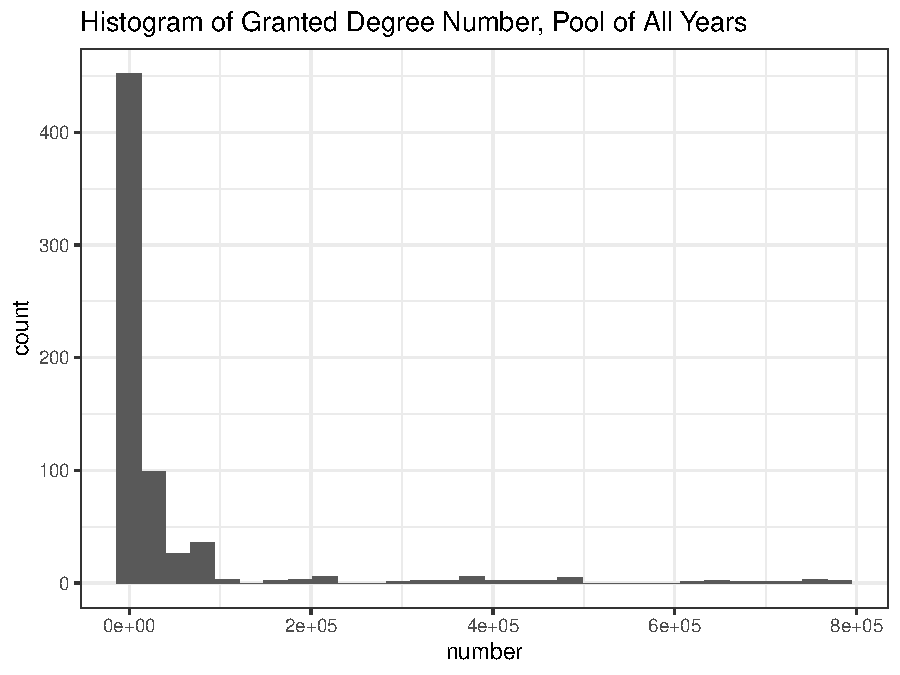
\includegraphics{hw1_sol_files/figure-latex/unnamed-chunk-7-1.pdf} \#\#
BS degrees in 2015

\begin{Shaded}
\begin{Highlighting}[]
\NormalTok{degreedata[,sci }\SpecialCharTok{:}\ErrorTok{=}\NormalTok{ field }\SpecialCharTok{!=} \StringTok{"Non{-}S\&E"}\NormalTok{]}

\NormalTok{degreedata.bs}\FloatTok{.2015} \OtherTok{=}\NormalTok{ degreedata[degree }\SpecialCharTok{==} \StringTok{"BS"} \SpecialCharTok{\&}\NormalTok{ year }\SpecialCharTok{==} \DecValTok{2015}\NormalTok{]}
\NormalTok{summary.bs}\FloatTok{.2015} \OtherTok{=} 
\NormalTok{  degreedata.bs}\FloatTok{.2015}\NormalTok{[,.(}\AttributeTok{number =} \FunctionTok{sum}\NormalTok{(number)),by }\OtherTok{=}\NormalTok{ .(sex,sci)]}
\NormalTok{summary.bs}\FloatTok{.2015}\NormalTok{[, percent }\SpecialCharTok{:}\ErrorTok{=}\NormalTok{ number}\SpecialCharTok{/}\FunctionTok{sum}\NormalTok{(number),by }\OtherTok{=}\NormalTok{ sci]}
\NormalTok{summary.bs.}\FloatTok{2015.}\NormalTok{wide }\OtherTok{=} \FunctionTok{data.frame}\NormalTok{(}\FunctionTok{acast}\NormalTok{(summary.bs}\FloatTok{.2015}\NormalTok{,sci}\SpecialCharTok{\textasciitilde{}}\NormalTok{sex,}\AttributeTok{value.var =} \StringTok{"number"}\NormalTok{))}
\FunctionTok{rownames}\NormalTok{(summary.bs.}\FloatTok{2015.}\NormalTok{wide) }\OtherTok{=} \FunctionTok{c}\NormalTok{(}\StringTok{"Non{-}sci"}\NormalTok{,}\StringTok{"Sci"}\NormalTok{)}
\NormalTok{summary.bs.}\FloatTok{2015.}\NormalTok{wide }\OtherTok{=} \FunctionTok{mutate}\NormalTok{(summary.bs.}\FloatTok{2015.}\NormalTok{wide,}\AttributeTok{Female.per =} 
                                \FunctionTok{paste}\NormalTok{(}\FunctionTok{sprintf}\NormalTok{(}\StringTok{\textquotesingle{}\%0.1f\textquotesingle{}}\NormalTok{,}\FunctionTok{round}\NormalTok{(summary.bs}\FloatTok{.2015}\SpecialCharTok{$}\NormalTok{percent[}\FunctionTok{c}\NormalTok{(}\DecValTok{2}\NormalTok{,}\DecValTok{1}\NormalTok{)]}\SpecialCharTok{*}\DecValTok{100}\NormalTok{,}\AttributeTok{digits =} \DecValTok{1}\NormalTok{)),}\StringTok{"\%"}\NormalTok{,}\AttributeTok{sep =} \StringTok{""}\NormalTok{))}

\CommentTok{\# summary table}
\FunctionTok{kbl}\NormalTok{(summary.bs.}\FloatTok{2015.}\NormalTok{wide, }\AttributeTok{caption =} \StringTok{"Summary Statistics for BS Degrees Granted in 2015 by Sex"}\NormalTok{, }\AttributeTok{digits =} \DecValTok{2}\NormalTok{, }\AttributeTok{booktabs =}\NormalTok{ T,}\AttributeTok{align =} \StringTok{"lccc"}\NormalTok{) }\SpecialCharTok{\%\textgreater{}\%}
  \FunctionTok{kable\_styling}\NormalTok{(}\AttributeTok{latex\_options =} \FunctionTok{c}\NormalTok{(}\StringTok{"HOLD\_position"}\NormalTok{))}\SpecialCharTok{\%\textgreater{}\%}
   \FunctionTok{footnote}\NormalTok{(}\AttributeTok{general =} \StringTok{"The table reports the summary statistics for the amount of BS degrees granted in 2015 by sex in the US degree data."}\NormalTok{,}
            \AttributeTok{threeparttable =}\NormalTok{ T)}
\end{Highlighting}
\end{Shaded}

\begin{table}[H]

\caption{\label{tab:unnamed-chunk-8}Summary Statistics for BS Degrees Granted in 2015 by Sex}
\centering
\begin{threeparttable}
\begin{tabular}[t]{llcc}
\toprule
  & Female & Male & Female.per\\
\midrule
Non-sci & 772768 & 493304 & 61.0\%\\
Sci & 322935 & 327122 & 49.7\%\\
\bottomrule
\end{tabular}
\begin{tablenotes}
\item \textit{Note: } 
\item The table reports the summary statistics for the amount of BS degrees granted in 2015 by sex in the US degree data.
\end{tablenotes}
\end{threeparttable}
\end{table}

\begin{Shaded}
\begin{Highlighting}[]
\CommentTok{\# bar plot}
\FunctionTok{ggplot}\NormalTok{(summary.bs}\FloatTok{.2015}\NormalTok{,}\FunctionTok{aes}\NormalTok{(}\AttributeTok{x=}\NormalTok{sci,}\AttributeTok{weight=}\NormalTok{number,}\AttributeTok{fill=}\NormalTok{sex))}\SpecialCharTok{+}
  \FunctionTok{geom\_bar}\NormalTok{(}\AttributeTok{color =} \StringTok{"black"}\NormalTok{, }\AttributeTok{width =}\NormalTok{ .}\DecValTok{7}\NormalTok{,}\AttributeTok{position =} \StringTok{\textquotesingle{}dodge\textquotesingle{}}\NormalTok{)}\SpecialCharTok{+}
  \FunctionTok{theme\_classic}\NormalTok{()}\SpecialCharTok{+}
  \FunctionTok{ylab}\NormalTok{(}\StringTok{\textquotesingle{}Number\textquotesingle{}}\NormalTok{)}\SpecialCharTok{+}
  \FunctionTok{xlab}\NormalTok{(}\StringTok{\textquotesingle{}Sci field\textquotesingle{}}\NormalTok{)}\SpecialCharTok{+}
  \FunctionTok{scale\_fill\_brewer}\NormalTok{(}\AttributeTok{palette =} \StringTok{"Set1"}\NormalTok{)}\SpecialCharTok{+}
  \FunctionTok{labs}\NormalTok{(}\AttributeTok{title =} \StringTok{"The Barplot of BS Degrees Granted in 2015, by Sex"}\NormalTok{)}
\end{Highlighting}
\end{Shaded}

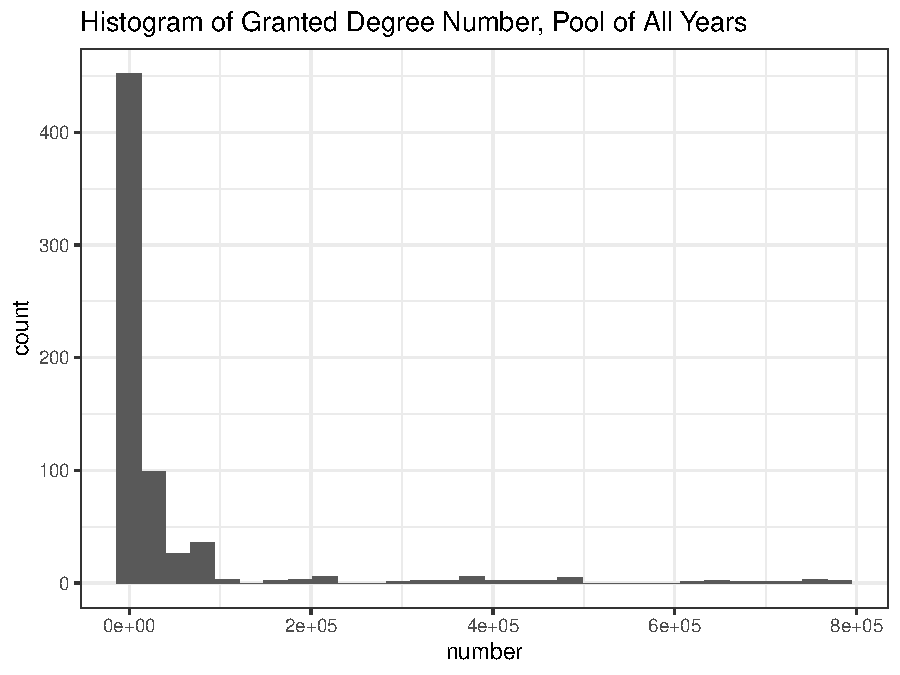
\includegraphics{hw1_sol_files/figure-latex/unnamed-chunk-8-1.pdf}

\hypertarget{bring-in-type-of-degree}{%
\subsection{Bring in Type of Degree}\label{bring-in-type-of-degree}}

\begin{Shaded}
\begin{Highlighting}[]
\NormalTok{summary.}\FloatTok{2015.}\NormalTok{sex.degree }\OtherTok{=}\NormalTok{ degreedata[year}\SpecialCharTok{==}\DecValTok{2015}\NormalTok{,}
\NormalTok{                          .(}\AttributeTok{number =} \FunctionTok{sum}\NormalTok{(number)),}
\NormalTok{                          by }\OtherTok{=}\NormalTok{ .(sex,degree)]}

\CommentTok{\# table}
\NormalTok{summary.}\FloatTok{2015.}\NormalTok{sex.degree.wide }\OtherTok{=} \FunctionTok{data.frame}\NormalTok{(}\FunctionTok{acast}\NormalTok{(summary.}\FloatTok{2015.}\NormalTok{sex.degree,degree}\SpecialCharTok{\textasciitilde{}}\NormalTok{sex))}
\end{Highlighting}
\end{Shaded}

\begin{verbatim}
## Using number as value column: use value.var to override.
\end{verbatim}

\begin{Shaded}
\begin{Highlighting}[]
\NormalTok{summary.}\FloatTok{2015.}\NormalTok{sex.degree.wide }\OtherTok{=} \FunctionTok{mutate}\NormalTok{(summary.}\FloatTok{2015.}\NormalTok{sex.degree.wide,}
                                      \AttributeTok{Female.per =} \FunctionTok{paste}\NormalTok{(}\FunctionTok{sprintf}\NormalTok{(}\StringTok{\textquotesingle{}\%0.1f\textquotesingle{}}\NormalTok{,}\FunctionTok{round}\NormalTok{(Female}\SpecialCharTok{/}\NormalTok{(Female}\SpecialCharTok{+}\NormalTok{Male)}\SpecialCharTok{*}\DecValTok{100}\NormalTok{,}\AttributeTok{digits =} \DecValTok{1}\NormalTok{)),}\StringTok{"\%"}\NormalTok{,}\AttributeTok{sep =} \StringTok{""}\NormalTok{))}
\FunctionTok{kbl}\NormalTok{(summary.}\FloatTok{2015.}\NormalTok{sex.degree.wide, }\AttributeTok{caption =} \StringTok{"Summary Statistics for Degrees Granted in 2015 by Sex"}\NormalTok{, }\AttributeTok{digits =} \DecValTok{2}\NormalTok{, }\AttributeTok{booktabs =}\NormalTok{ T,}\AttributeTok{align =} \StringTok{"lccc"}\NormalTok{) }\SpecialCharTok{\%\textgreater{}\%}
  \FunctionTok{kable\_styling}\NormalTok{(}\AttributeTok{latex\_options =} \FunctionTok{c}\NormalTok{(}\StringTok{"HOLD\_position"}\NormalTok{))}\SpecialCharTok{\%\textgreater{}\%}
   \FunctionTok{footnote}\NormalTok{(}\AttributeTok{general =} \StringTok{"The table reports the summary statistics for the amount of degrees granted in 2015 by sex in the US degree data."}\NormalTok{,}
            \AttributeTok{threeparttable =}\NormalTok{ T)}
\end{Highlighting}
\end{Shaded}

\begin{table}[H]

\caption{\label{tab:unnamed-chunk-9}Summary Statistics for Degrees Granted in 2015 by Sex}
\centering
\begin{threeparttable}
\begin{tabular}[t]{llcc}
\toprule
  & Female & Male & Female.per\\
\midrule
BS & 1095703 & 820426 & 57.2\%\\
MS & 455697 & 308283 & 59.6\%\\
PhD & 34660 & 34455 & 50.1\%\\
\bottomrule
\end{tabular}
\begin{tablenotes}
\item \textit{Note: } 
\item The table reports the summary statistics for the amount of degrees granted in 2015 by sex in the US degree data.
\end{tablenotes}
\end{threeparttable}
\end{table}

\begin{Shaded}
\begin{Highlighting}[]
\CommentTok{\# barplot}
\FunctionTok{ggplot}\NormalTok{(summary.}\FloatTok{2015.}\NormalTok{sex.degree,}\FunctionTok{aes}\NormalTok{(}\AttributeTok{x=}\NormalTok{degree,}\AttributeTok{weight=}\NormalTok{number,}\AttributeTok{fill=}\NormalTok{sex))}\SpecialCharTok{+}
  \FunctionTok{geom\_bar}\NormalTok{(}\AttributeTok{color =} \StringTok{"black"}\NormalTok{, }\AttributeTok{width =}\NormalTok{ .}\DecValTok{7}\NormalTok{,}\AttributeTok{position =} \StringTok{\textquotesingle{}dodge\textquotesingle{}}\NormalTok{)}\SpecialCharTok{+}
  \FunctionTok{theme\_classic}\NormalTok{()}\SpecialCharTok{+}
  \FunctionTok{ylab}\NormalTok{(}\StringTok{\textquotesingle{}Number\textquotesingle{}}\NormalTok{)}\SpecialCharTok{+}
  \FunctionTok{xlab}\NormalTok{(}\StringTok{\textquotesingle{}Degree\textquotesingle{}}\NormalTok{)}\SpecialCharTok{+}
  \FunctionTok{scale\_fill\_brewer}\NormalTok{(}\AttributeTok{palette =} \StringTok{"Set1"}\NormalTok{)}\SpecialCharTok{+}
  \FunctionTok{labs}\NormalTok{(}\AttributeTok{title =} \StringTok{"The Barplot of Degrees Granted in 2015, by Sex"}\NormalTok{)}
\end{Highlighting}
\end{Shaded}

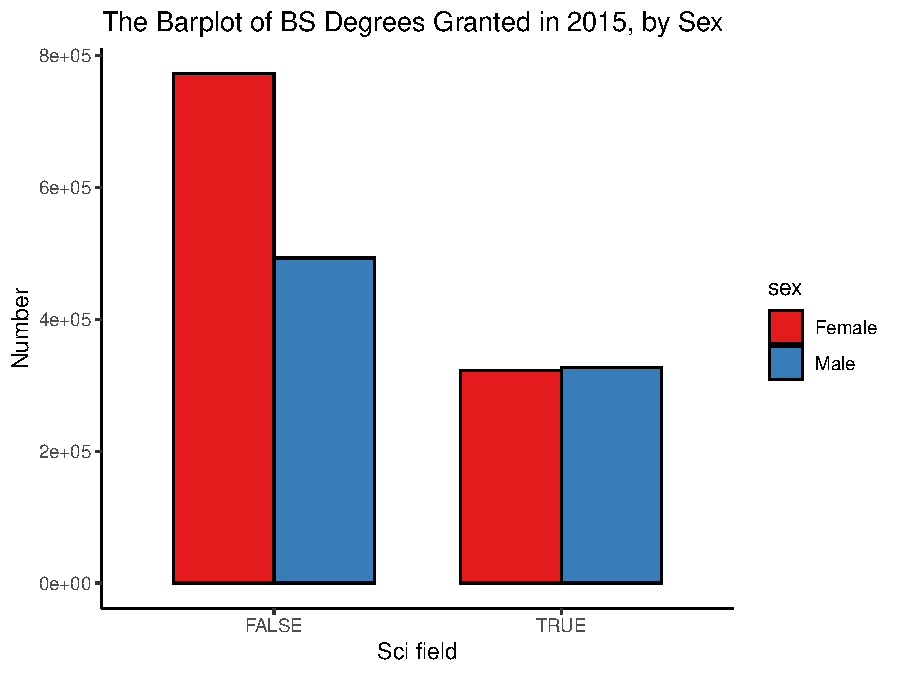
\includegraphics{hw1_sol_files/figure-latex/unnamed-chunk-9-1.pdf}

\hypertarget{bring-all-variables}{%
\subsection{Bring All Variables}\label{bring-all-variables}}

\begin{Shaded}
\begin{Highlighting}[]
\NormalTok{summary.sex.time }\OtherTok{=}\NormalTok{ degreedata[,}
\NormalTok{                          .(}\AttributeTok{number =} \FunctionTok{sum}\NormalTok{(number)),}
\NormalTok{                          by }\OtherTok{=}\NormalTok{ .(sex,year)]}
\NormalTok{summary.sex.time[,percent }\SpecialCharTok{:}\ErrorTok{=}\NormalTok{ number}\SpecialCharTok{/}\FunctionTok{sum}\NormalTok{(number),by }\OtherTok{=}\NormalTok{ year]}

\CommentTok{\# table}
\NormalTok{summary.sex.time.wide }\OtherTok{=} \FunctionTok{data.frame}\NormalTok{(}\FunctionTok{acast}\NormalTok{(summary.sex.time,year}\SpecialCharTok{\textasciitilde{}}\NormalTok{sex,}\AttributeTok{value.var =} \StringTok{"number"}\NormalTok{))}
\NormalTok{summary.sex.time.wide }\OtherTok{=} \FunctionTok{mutate}\NormalTok{(summary.sex.time.wide,}
                                      \AttributeTok{Female.per =} \FunctionTok{paste}\NormalTok{(}\FunctionTok{sprintf}\NormalTok{(}\StringTok{\textquotesingle{}\%0.1f\textquotesingle{}}\NormalTok{,}\FunctionTok{round}\NormalTok{(Female}\SpecialCharTok{/}\NormalTok{(Female}\SpecialCharTok{+}\NormalTok{Male)}\SpecialCharTok{*}\DecValTok{100}\NormalTok{,}\AttributeTok{digits =} \DecValTok{1}\NormalTok{)),}\StringTok{"\%"}\NormalTok{,}\AttributeTok{sep =} \StringTok{""}\NormalTok{))}
\FunctionTok{kbl}\NormalTok{(summary.sex.time.wide, }\AttributeTok{caption =} \StringTok{"Summary Statistics for Degrees Granted by Sex, 2006{-}2016"}\NormalTok{, }\AttributeTok{digits =} \DecValTok{2}\NormalTok{, }\AttributeTok{booktabs =}\NormalTok{ T,}\AttributeTok{align =} \StringTok{"lccc"}\NormalTok{) }\SpecialCharTok{\%\textgreater{}\%}
  \FunctionTok{kable\_styling}\NormalTok{(}\AttributeTok{latex\_options =} \FunctionTok{c}\NormalTok{(}\StringTok{"HOLD\_position"}\NormalTok{))}\SpecialCharTok{\%\textgreater{}\%}
   \FunctionTok{footnote}\NormalTok{(}\AttributeTok{general =} \StringTok{"The table reports the summary statistics for the amount of degrees granted within 2006{-}2016 by sex in the US degree data."}\NormalTok{,}
            \AttributeTok{threeparttable =}\NormalTok{ T)}
\end{Highlighting}
\end{Shaded}

\begin{table}[H]

\caption{\label{tab:unnamed-chunk-10}Summary Statistics for Degrees Granted by Sex, 2006-2016}
\centering
\begin{threeparttable}
\begin{tabular}[t]{llcc}
\toprule
  & Female & Male & Female.per\\
\midrule
2006 & 1253917 & 904679 & 58.1\%\\
2007 & 1287439 & 925621 & 58.2\%\\
2008 & 1320480 & 953360 & 58.1\%\\
2009 & 1360820 & 985411 & 58.0\%\\
2010 & 1404646 & 1019514 & 57.9\%\\
\addlinespace
2011 & 1466539 & 1063992 & 58.0\%\\
2012 & 1525402 & 1107721 & 57.9\%\\
2013 & 1552075 & 1130821 & 57.9\%\\
2014 & 1570559 & 1147769 & 57.8\%\\
2015 & 1586060 & 1163164 & 57.7\%\\
\addlinespace
2016 & 1616307 & 1186906 & 57.7\%\\
\bottomrule
\end{tabular}
\begin{tablenotes}
\item \textit{Note: } 
\item The table reports the summary statistics for the amount of degrees granted within 2006-2016 by sex in the US degree data.
\end{tablenotes}
\end{threeparttable}
\end{table}

\begin{Shaded}
\begin{Highlighting}[]
\CommentTok{\# barplot}
\FunctionTok{ggplot}\NormalTok{()}\SpecialCharTok{+}
  \FunctionTok{geom\_bar}\NormalTok{(}\AttributeTok{data =}\NormalTok{ summary.sex.time,}\FunctionTok{aes}\NormalTok{(}\AttributeTok{x=}\FunctionTok{as.factor}\NormalTok{(year),}\AttributeTok{weight=}\NormalTok{number,}\AttributeTok{fill=}\NormalTok{sex),}
           \AttributeTok{color =} \StringTok{"black"}\NormalTok{, }\AttributeTok{width =}\NormalTok{ .}\DecValTok{7}\NormalTok{,}\AttributeTok{position =} \StringTok{\textquotesingle{}dodge\textquotesingle{}}\NormalTok{)}\SpecialCharTok{+}
  \FunctionTok{theme\_classic}\NormalTok{()}\SpecialCharTok{+}
  \FunctionTok{ylab}\NormalTok{(}\StringTok{\textquotesingle{}Number\textquotesingle{}}\NormalTok{)}\SpecialCharTok{+}
  \FunctionTok{scale\_y\_continuous}\NormalTok{(}\AttributeTok{limits =} \FunctionTok{c}\NormalTok{(}\DecValTok{0}\NormalTok{,}\DecValTok{2000000}\NormalTok{),}
                     \AttributeTok{sec.axis =} \FunctionTok{sec\_axis}\NormalTok{(}\SpecialCharTok{\textasciitilde{}}\NormalTok{.}\SpecialCharTok{/}\DecValTok{10000000}\FloatTok{+0.4}\NormalTok{, }\AttributeTok{name =} \StringTok{"Female Percent"}\NormalTok{))}\SpecialCharTok{+}
  \FunctionTok{geom\_line}\NormalTok{(}\AttributeTok{data =}\NormalTok{ summary.sex.time[sex}\SpecialCharTok{==}\StringTok{"Female"}\NormalTok{],}
            \FunctionTok{aes}\NormalTok{(}\AttributeTok{x=}\FunctionTok{as.factor}\NormalTok{(year),}\AttributeTok{y=}\DecValTok{10000000}\SpecialCharTok{*}\NormalTok{(percent}\FloatTok{{-}0.4}\NormalTok{),}\AttributeTok{group=}\DecValTok{1}\NormalTok{))}\SpecialCharTok{+}
  \FunctionTok{xlab}\NormalTok{(}\StringTok{\textquotesingle{}Year\textquotesingle{}}\NormalTok{)}\SpecialCharTok{+}
  \FunctionTok{scale\_fill\_brewer}\NormalTok{(}\AttributeTok{palette =} \StringTok{"Set1"}\NormalTok{)}\SpecialCharTok{+}
  \FunctionTok{labs}\NormalTok{(}\AttributeTok{title =} \StringTok{"The Barplot of Degrees Granted in 2006{-}2016, by Sex"}\NormalTok{)}
\end{Highlighting}
\end{Shaded}

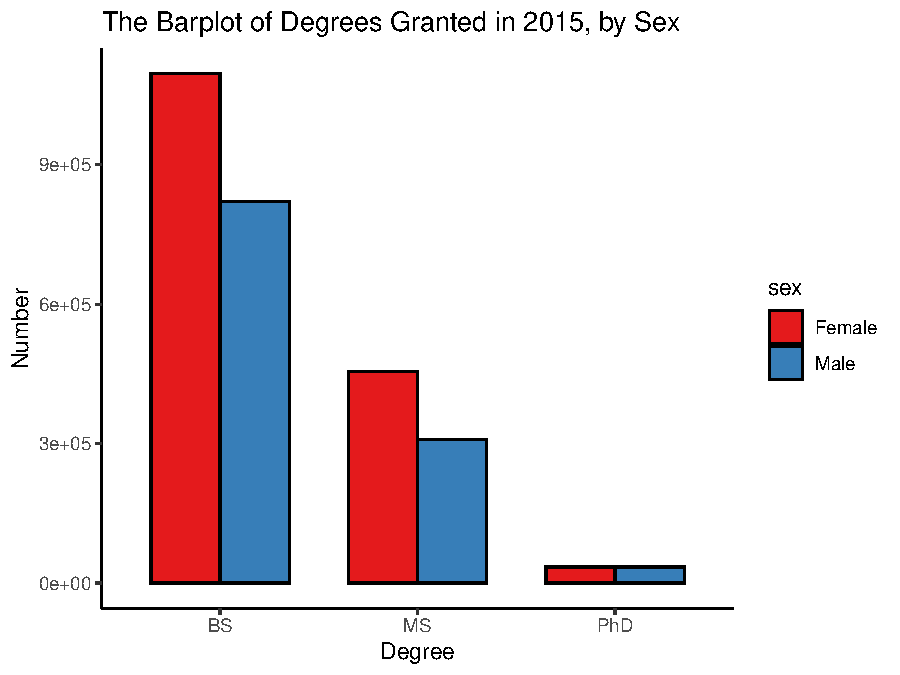
\includegraphics{hw1_sol_files/figure-latex/unnamed-chunk-10-1.pdf} \#\#
Focus on Data Science

\begin{Shaded}
\begin{Highlighting}[]
\NormalTok{degreedata[, datasci }\SpecialCharTok{:}\ErrorTok{=}\NormalTok{ field }\SpecialCharTok{\%in\%} \FunctionTok{c}\NormalTok{(}\StringTok{"Computer sciences"}\NormalTok{,}\StringTok{"Mathematics and statistics"}\NormalTok{)]}
\NormalTok{summary.ds }\OtherTok{=}\NormalTok{ degreedata[,}
\NormalTok{                             .(}\AttributeTok{number =} \FunctionTok{sum}\NormalTok{(number)),}
\NormalTok{                             by }\OtherTok{=}\NormalTok{ .(sci,datasci,sex,year)]}
\NormalTok{summary.ds.timeagg }\OtherTok{=}\NormalTok{ summary.ds[,.(}\AttributeTok{number =} \FunctionTok{sum}\NormalTok{(number)),by }\OtherTok{=}\NormalTok{ .(sci,datasci,sex)]}
\NormalTok{summary.ds.timeagg[, percent }\SpecialCharTok{:}\ErrorTok{=}\NormalTok{ number}\SpecialCharTok{/}\FunctionTok{sum}\NormalTok{(number),by }\OtherTok{=}\NormalTok{ .(datasci,sci)]}

\CommentTok{\# sci vs non{-}sci: we have conclusions before. We want to know whether it\textquotesingle{}s more severe in ds compared to other sci.}
\NormalTok{summary.ds.timeagg.wide }\OtherTok{=} \FunctionTok{data.frame}\NormalTok{(}\FunctionTok{acast}\NormalTok{(summary.ds.timeagg[sci}\SpecialCharTok{==}\NormalTok{T],datasci}\SpecialCharTok{\textasciitilde{}}\NormalTok{sex,}\AttributeTok{value.var =} \StringTok{"number"}\NormalTok{))}
\FunctionTok{rownames}\NormalTok{(summary.ds.timeagg.wide) }\OtherTok{=} \FunctionTok{c}\NormalTok{(}\StringTok{"non{-}data sci"}\NormalTok{,}\StringTok{" data sci"}\NormalTok{)}
\NormalTok{summary.ds.timeagg.wide }\OtherTok{=} \FunctionTok{mutate}\NormalTok{(summary.ds.timeagg.wide,}\AttributeTok{Female.per =} 
                                \FunctionTok{paste}\NormalTok{(}\FunctionTok{sprintf}\NormalTok{(}\StringTok{\textquotesingle{}\%0.1f\textquotesingle{}}\NormalTok{,}\FunctionTok{round}\NormalTok{(summary.ds.timeagg}\SpecialCharTok{$}\NormalTok{percent[}\DecValTok{1}\SpecialCharTok{:}\DecValTok{2}\NormalTok{]}\SpecialCharTok{*}\DecValTok{100}\NormalTok{,}\AttributeTok{digits =} \DecValTok{1}\NormalTok{)),}\StringTok{"\%"}\NormalTok{,}\AttributeTok{sep =} \StringTok{""}\NormalTok{))}

\CommentTok{\# summary table}
\FunctionTok{kbl}\NormalTok{(summary.ds.timeagg.wide, }\AttributeTok{caption =} \StringTok{"Summary Statistics for Degrees Granted in SCI Field by Sex"}\NormalTok{, }\AttributeTok{digits =} \DecValTok{2}\NormalTok{, }\AttributeTok{booktabs =}\NormalTok{ T,}\AttributeTok{align =} \StringTok{"lccc"}\NormalTok{) }\SpecialCharTok{\%\textgreater{}\%}
  \FunctionTok{kable\_styling}\NormalTok{(}\AttributeTok{latex\_options =} \FunctionTok{c}\NormalTok{(}\StringTok{"HOLD\_position"}\NormalTok{))}\SpecialCharTok{\%\textgreater{}\%}
   \FunctionTok{footnote}\NormalTok{(}\AttributeTok{general =} \StringTok{"The table reports the summary statistics for the amount of sci degrees granted over the sample period, separated by sex and data science or not."}\NormalTok{,}
            \AttributeTok{threeparttable =}\NormalTok{ T)}
\end{Highlighting}
\end{Shaded}

\begin{table}[H]

\caption{\label{tab:unnamed-chunk-11}Summary Statistics for Degrees Granted in SCI Field by Sex}
\centering
\begin{threeparttable}
\begin{tabular}[t]{llcc}
\toprule
  & Female & Male & Female.per\\
\midrule
non-data sci & 3731029 & 3432349 & 52.1\%\\
data sci & 296891 & 799889 & 27.1\%\\
\bottomrule
\end{tabular}
\begin{tablenotes}
\item \textit{Note: } 
\item The table reports the summary statistics for the amount of sci degrees granted over the sample period, separated by sex and data science or not.
\end{tablenotes}
\end{threeparttable}
\end{table}

\begin{Shaded}
\begin{Highlighting}[]
\CommentTok{\# barplot}
\FunctionTok{ggplot}\NormalTok{(summary.ds.timeagg[sci}\SpecialCharTok{==}\NormalTok{T],}\FunctionTok{aes}\NormalTok{(}\AttributeTok{x=}\NormalTok{datasci,}\AttributeTok{weight=}\NormalTok{number,}\AttributeTok{fill=}\NormalTok{sex))}\SpecialCharTok{+}
  \FunctionTok{geom\_bar}\NormalTok{(}\AttributeTok{color =} \StringTok{"black"}\NormalTok{, }\AttributeTok{width =}\NormalTok{ .}\DecValTok{7}\NormalTok{,}\AttributeTok{position =} \StringTok{\textquotesingle{}dodge\textquotesingle{}}\NormalTok{)}\SpecialCharTok{+}
  \FunctionTok{theme\_classic}\NormalTok{()}\SpecialCharTok{+}
  \FunctionTok{ylab}\NormalTok{(}\StringTok{\textquotesingle{}Number\textquotesingle{}}\NormalTok{)}\SpecialCharTok{+}
  \FunctionTok{xlab}\NormalTok{(}\StringTok{\textquotesingle{}data science\textquotesingle{}}\NormalTok{)}\SpecialCharTok{+}
  \FunctionTok{scale\_fill\_brewer}\NormalTok{(}\AttributeTok{palette =} \StringTok{"Set1"}\NormalTok{)}\SpecialCharTok{+}
  \FunctionTok{labs}\NormalTok{(}\AttributeTok{title =} \StringTok{"The Barplot of Degrees Granted in SCI Field, by Sex"}\NormalTok{)}
\end{Highlighting}
\end{Shaded}

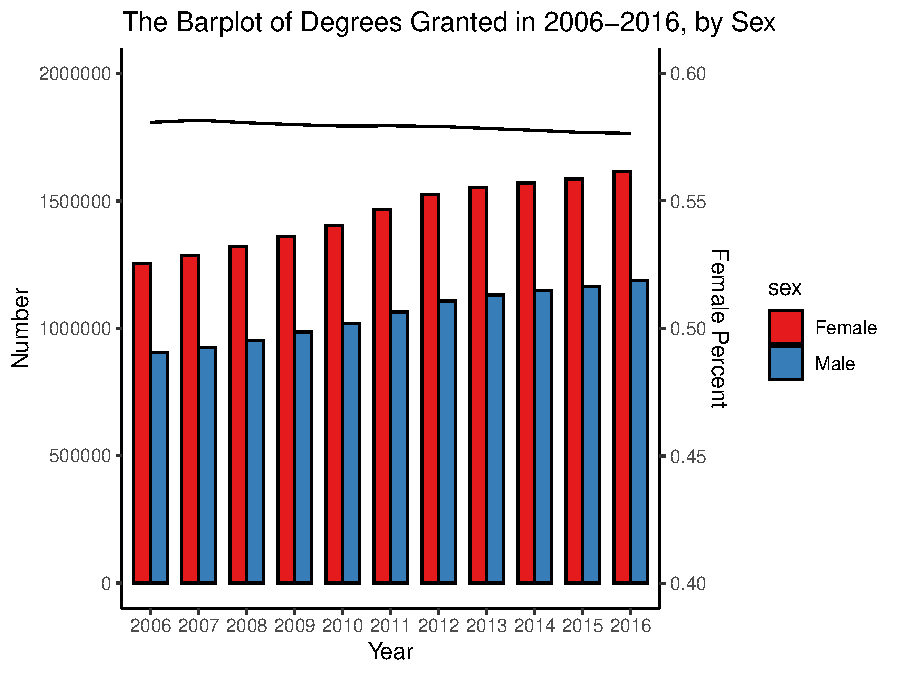
\includegraphics{hw1_sol_files/figure-latex/unnamed-chunk-11-1.pdf}

\hypertarget{by-degree}{%
\subsubsection{By Degree}\label{by-degree}}

\begin{Shaded}
\begin{Highlighting}[]
\DocumentationTok{\#\# }
\NormalTok{summary.ds.bs }\OtherTok{=}\NormalTok{ degreedata[sci}\SpecialCharTok{==}\ConstantTok{TRUE}\SpecialCharTok{\&}\NormalTok{degree}\SpecialCharTok{==}\StringTok{"BS"}\NormalTok{,.(}
  \AttributeTok{number =} \FunctionTok{sum}\NormalTok{(number)}
\NormalTok{), by }\OtherTok{=}\NormalTok{ .(datasci,sex)]}
\NormalTok{summary.ds.bs[, percent }\SpecialCharTok{:}\ErrorTok{=}\NormalTok{ number}\SpecialCharTok{/}\FunctionTok{sum}\NormalTok{(number),by }\OtherTok{=}\NormalTok{ .(datasci)]}
\NormalTok{summary.ds.ms }\OtherTok{=}\NormalTok{ degreedata[sci}\SpecialCharTok{==}\ConstantTok{TRUE}\SpecialCharTok{\&}\NormalTok{degree}\SpecialCharTok{==}\StringTok{"MS"}\NormalTok{,.(}
  \AttributeTok{number =} \FunctionTok{sum}\NormalTok{(number)}
\NormalTok{), by }\OtherTok{=}\NormalTok{ .(datasci,sex)]}
\NormalTok{summary.ds.ms[, percent }\SpecialCharTok{:}\ErrorTok{=}\NormalTok{ number}\SpecialCharTok{/}\FunctionTok{sum}\NormalTok{(number),by }\OtherTok{=}\NormalTok{ .(datasci)]}
\NormalTok{summary.ds.phd }\OtherTok{=}\NormalTok{ degreedata[sci}\SpecialCharTok{==}\ConstantTok{TRUE}\SpecialCharTok{\&}\NormalTok{degree}\SpecialCharTok{==}\StringTok{"PhD"}\NormalTok{,.(}
  \AttributeTok{number =} \FunctionTok{sum}\NormalTok{(number)}
\NormalTok{), by }\OtherTok{=}\NormalTok{ .(datasci,sex)]}
\NormalTok{summary.ds.phd[, percent }\SpecialCharTok{:}\ErrorTok{=}\NormalTok{ number}\SpecialCharTok{/}\FunctionTok{sum}\NormalTok{(number),by }\OtherTok{=}\NormalTok{ .(datasci)]}

\CommentTok{\# sci vs non{-}sci: we have conclusions before. We want to know whether it\textquotesingle{}s more severe in ds compared to other sci.}
\NormalTok{summary.ds.bs.wide }\OtherTok{=} \FunctionTok{data.frame}\NormalTok{(}\FunctionTok{acast}\NormalTok{(summary.ds.bs,datasci}\SpecialCharTok{\textasciitilde{}}\NormalTok{sex,}\AttributeTok{value.var =} \StringTok{"number"}\NormalTok{))}
\FunctionTok{rownames}\NormalTok{(summary.ds.bs.wide) }\OtherTok{=} \FunctionTok{c}\NormalTok{(}\StringTok{"non{-}data sci"}\NormalTok{,}\StringTok{" data sci"}\NormalTok{)}
\NormalTok{summary.ds.bs.wide }\OtherTok{=} \FunctionTok{mutate}\NormalTok{(summary.ds.bs.wide,}\AttributeTok{Female.per =} 
                                \FunctionTok{paste}\NormalTok{(}\FunctionTok{sprintf}\NormalTok{(}\StringTok{\textquotesingle{}\%0.1f\textquotesingle{}}\NormalTok{,}\FunctionTok{round}\NormalTok{(summary.ds.bs}\SpecialCharTok{$}\NormalTok{percent[}\DecValTok{1}\SpecialCharTok{:}\DecValTok{2}\NormalTok{]}\SpecialCharTok{*}\DecValTok{100}\NormalTok{,}\AttributeTok{digits =} \DecValTok{1}\NormalTok{)),}\StringTok{"\%"}\NormalTok{,}\AttributeTok{sep =} \StringTok{""}\NormalTok{))}
\NormalTok{summary.ds.ms.wide }\OtherTok{=} \FunctionTok{data.frame}\NormalTok{(}\FunctionTok{acast}\NormalTok{(summary.ds.ms,datasci}\SpecialCharTok{\textasciitilde{}}\NormalTok{sex,}\AttributeTok{value.var =} \StringTok{"number"}\NormalTok{))}
\FunctionTok{rownames}\NormalTok{(summary.ds.ms.wide) }\OtherTok{=} \FunctionTok{c}\NormalTok{(}\StringTok{"non{-}data sci"}\NormalTok{,}\StringTok{" data sci"}\NormalTok{)}
\NormalTok{summary.ds.ms.wide }\OtherTok{=} \FunctionTok{mutate}\NormalTok{(summary.ds.ms.wide,}\AttributeTok{Female.per =} 
                                \FunctionTok{paste}\NormalTok{(}\FunctionTok{sprintf}\NormalTok{(}\StringTok{\textquotesingle{}\%0.1f\textquotesingle{}}\NormalTok{,}\FunctionTok{round}\NormalTok{(summary.ds.ms}\SpecialCharTok{$}\NormalTok{percent[}\DecValTok{1}\SpecialCharTok{:}\DecValTok{2}\NormalTok{]}\SpecialCharTok{*}\DecValTok{100}\NormalTok{,}\AttributeTok{digits =} \DecValTok{1}\NormalTok{)),}\StringTok{"\%"}\NormalTok{,}\AttributeTok{sep =} \StringTok{""}\NormalTok{))}
\NormalTok{summary.ds.phd.wide }\OtherTok{=} \FunctionTok{data.frame}\NormalTok{(}\FunctionTok{acast}\NormalTok{(summary.ds.phd,datasci}\SpecialCharTok{\textasciitilde{}}\NormalTok{sex,}\AttributeTok{value.var =} \StringTok{"number"}\NormalTok{))}
\FunctionTok{rownames}\NormalTok{(summary.ds.phd.wide) }\OtherTok{=} \FunctionTok{c}\NormalTok{(}\StringTok{"non{-}data sci"}\NormalTok{,}\StringTok{" data sci"}\NormalTok{)}
\NormalTok{summary.ds.phd.wide }\OtherTok{=} \FunctionTok{mutate}\NormalTok{(summary.ds.phd.wide,}\AttributeTok{Female.per =} 
                                \FunctionTok{paste}\NormalTok{(}\FunctionTok{sprintf}\NormalTok{(}\StringTok{\textquotesingle{}\%0.1f\textquotesingle{}}\NormalTok{,}\FunctionTok{round}\NormalTok{(summary.ds.phd}\SpecialCharTok{$}\NormalTok{percent[}\DecValTok{1}\SpecialCharTok{:}\DecValTok{2}\NormalTok{]}\SpecialCharTok{*}\DecValTok{100}\NormalTok{,}\AttributeTok{digits =} \DecValTok{1}\NormalTok{)),}\StringTok{"\%"}\NormalTok{,}\AttributeTok{sep =} \StringTok{""}\NormalTok{))}

\CommentTok{\# summary table}
\FunctionTok{kbl}\NormalTok{(summary.ds.bs.wide, }\AttributeTok{caption =} \StringTok{"Summary Statistics for BS Degrees Granted in SCI Field by Sex"}\NormalTok{, }\AttributeTok{digits =} \DecValTok{2}\NormalTok{, }\AttributeTok{booktabs =}\NormalTok{ T,}\AttributeTok{align =} \StringTok{"lccc"}\NormalTok{) }\SpecialCharTok{\%\textgreater{}\%}
  \FunctionTok{kable\_styling}\NormalTok{(}\AttributeTok{latex\_options =} \FunctionTok{c}\NormalTok{(}\StringTok{"HOLD\_position"}\NormalTok{))}\SpecialCharTok{\%\textgreater{}\%}
   \FunctionTok{footnote}\NormalTok{(}\AttributeTok{general =} \StringTok{"The table reports the summary statistics for the amount of BS sci degrees granted over the sample period, separated by sex and data science or not."}\NormalTok{,}
            \AttributeTok{threeparttable =}\NormalTok{ T)}
\end{Highlighting}
\end{Shaded}

\begin{table}[H]

\caption{\label{tab:unnamed-chunk-12}Summary Statistics for BS Degrees Granted in SCI Field by Sex}
\centering
\begin{threeparttable}
\begin{tabular}[t]{llcc}
\toprule
  & Female & Male & Female.per\\
\midrule
non-data sci & 2923482 & 2537905 & 53.5\%\\
data sci & 188047 & 553709 & 25.4\%\\
\bottomrule
\end{tabular}
\begin{tablenotes}
\item \textit{Note: } 
\item The table reports the summary statistics for the amount of BS sci degrees granted over the sample period, separated by sex and data science or not.
\end{tablenotes}
\end{threeparttable}
\end{table}

\begin{Shaded}
\begin{Highlighting}[]
\FunctionTok{kbl}\NormalTok{(summary.ds.ms.wide, }\AttributeTok{caption =} \StringTok{"Summary Statistics for MS Degrees Granted in SCI Field by Sex"}\NormalTok{, }\AttributeTok{digits =} \DecValTok{2}\NormalTok{, }\AttributeTok{booktabs =}\NormalTok{ T,}\AttributeTok{align =} \StringTok{"lccc"}\NormalTok{) }\SpecialCharTok{\%\textgreater{}\%}
  \FunctionTok{kable\_styling}\NormalTok{(}\AttributeTok{latex\_options =} \FunctionTok{c}\NormalTok{(}\StringTok{"HOLD\_position"}\NormalTok{))}\SpecialCharTok{\%\textgreater{}\%}
   \FunctionTok{footnote}\NormalTok{(}\AttributeTok{general =} \StringTok{"The table reports the summary statistics for the amount of MS sci degrees granted over the sample period, separated by sex and data science or not."}\NormalTok{,}
            \AttributeTok{threeparttable =}\NormalTok{ T)}
\end{Highlighting}
\end{Shaded}

\begin{table}[H]

\caption{\label{tab:unnamed-chunk-12}Summary Statistics for MS Degrees Granted in SCI Field by Sex}
\centering
\begin{threeparttable}
\begin{tabular}[t]{llcc}
\toprule
  & Female & Male & Female.per\\
\midrule
non-data sci & 658613 & 693861 & 48.7\%\\
data sci & 99704 & 218843 & 31.3\%\\
\bottomrule
\end{tabular}
\begin{tablenotes}
\item \textit{Note: } 
\item The table reports the summary statistics for the amount of MS sci degrees granted over the sample period, separated by sex and data science or not.
\end{tablenotes}
\end{threeparttable}
\end{table}

\begin{Shaded}
\begin{Highlighting}[]
\FunctionTok{kbl}\NormalTok{(summary.ds.phd.wide, }\AttributeTok{caption =} \StringTok{"Summary Statistics for PhD Degrees Granted in SCI Field by Sex"}\NormalTok{, }\AttributeTok{digits =} \DecValTok{2}\NormalTok{, }\AttributeTok{booktabs =}\NormalTok{ T,}\AttributeTok{align =} \StringTok{"lccc"}\NormalTok{) }\SpecialCharTok{\%\textgreater{}\%}
  \FunctionTok{kable\_styling}\NormalTok{(}\AttributeTok{latex\_options =} \FunctionTok{c}\NormalTok{(}\StringTok{"HOLD\_position"}\NormalTok{))}\SpecialCharTok{\%\textgreater{}\%}
   \FunctionTok{footnote}\NormalTok{(}\AttributeTok{general =} \StringTok{"The table reports the summary statistics for the amount of PhD sci degrees granted over the sample period, separated by sex and data science or not."}\NormalTok{,}
            \AttributeTok{threeparttable =}\NormalTok{ T)}
\end{Highlighting}
\end{Shaded}

\begin{table}[H]

\caption{\label{tab:unnamed-chunk-12}Summary Statistics for PhD Degrees Granted in SCI Field by Sex}
\centering
\begin{threeparttable}
\begin{tabular}[t]{llcc}
\toprule
  & Female & Male & Female.per\\
\midrule
non-data sci & 148934 & 200583 & 42.6\%\\
data sci & 9140 & 27337 & 25.1\%\\
\bottomrule
\end{tabular}
\begin{tablenotes}
\item \textit{Note: } 
\item The table reports the summary statistics for the amount of PhD sci degrees granted over the sample period, separated by sex and data science or not.
\end{tablenotes}
\end{threeparttable}
\end{table}

\begin{Shaded}
\begin{Highlighting}[]
\CommentTok{\# barplot}
\FunctionTok{ggplot}\NormalTok{(summary.ds.bs,}\FunctionTok{aes}\NormalTok{(}\AttributeTok{x=}\NormalTok{datasci,}\AttributeTok{weight=}\NormalTok{number,}\AttributeTok{fill=}\NormalTok{sex))}\SpecialCharTok{+}
  \FunctionTok{geom\_bar}\NormalTok{(}\AttributeTok{color =} \StringTok{"black"}\NormalTok{, }\AttributeTok{width =}\NormalTok{ .}\DecValTok{7}\NormalTok{,}\AttributeTok{position =} \StringTok{\textquotesingle{}dodge\textquotesingle{}}\NormalTok{)}\SpecialCharTok{+}
  \FunctionTok{theme\_classic}\NormalTok{()}\SpecialCharTok{+}
  \FunctionTok{ylab}\NormalTok{(}\StringTok{\textquotesingle{}Number\textquotesingle{}}\NormalTok{)}\SpecialCharTok{+}
  \FunctionTok{xlab}\NormalTok{(}\StringTok{\textquotesingle{}data science\textquotesingle{}}\NormalTok{)}\SpecialCharTok{+}
  \FunctionTok{scale\_fill\_brewer}\NormalTok{(}\AttributeTok{palette =} \StringTok{"Set1"}\NormalTok{)}\SpecialCharTok{+}
  \FunctionTok{labs}\NormalTok{(}\AttributeTok{title =} \StringTok{"The Barplot of BS Degrees Granted in SCI Field, by Sex"}\NormalTok{)}
\end{Highlighting}
\end{Shaded}

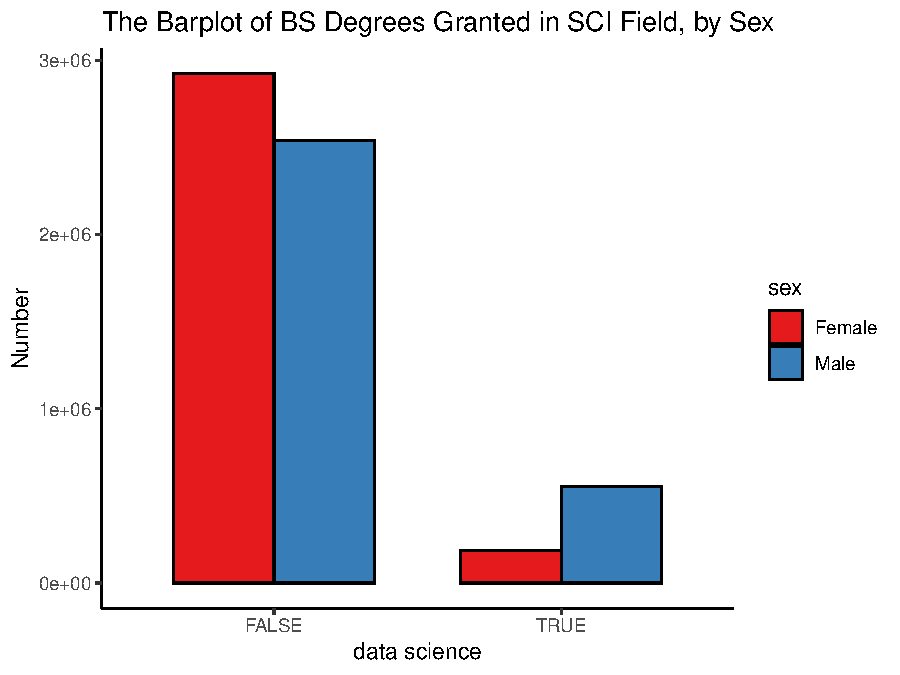
\includegraphics{hw1_sol_files/figure-latex/unnamed-chunk-12-1.pdf}

\begin{Shaded}
\begin{Highlighting}[]
\FunctionTok{ggplot}\NormalTok{(summary.ds.ms,}\FunctionTok{aes}\NormalTok{(}\AttributeTok{x=}\NormalTok{datasci,}\AttributeTok{weight=}\NormalTok{number,}\AttributeTok{fill=}\NormalTok{sex))}\SpecialCharTok{+}
  \FunctionTok{geom\_bar}\NormalTok{(}\AttributeTok{color =} \StringTok{"black"}\NormalTok{, }\AttributeTok{width =}\NormalTok{ .}\DecValTok{7}\NormalTok{,}\AttributeTok{position =} \StringTok{\textquotesingle{}dodge\textquotesingle{}}\NormalTok{)}\SpecialCharTok{+}
  \FunctionTok{theme\_classic}\NormalTok{()}\SpecialCharTok{+}
  \FunctionTok{ylab}\NormalTok{(}\StringTok{\textquotesingle{}Number\textquotesingle{}}\NormalTok{)}\SpecialCharTok{+}
  \FunctionTok{xlab}\NormalTok{(}\StringTok{\textquotesingle{}data science\textquotesingle{}}\NormalTok{)}\SpecialCharTok{+}
  \FunctionTok{scale\_fill\_brewer}\NormalTok{(}\AttributeTok{palette =} \StringTok{"Set1"}\NormalTok{)}\SpecialCharTok{+}
  \FunctionTok{labs}\NormalTok{(}\AttributeTok{title =} \StringTok{"The Barplot of MS Degrees Granted in SCI Field, by Sex"}\NormalTok{)}
\end{Highlighting}
\end{Shaded}

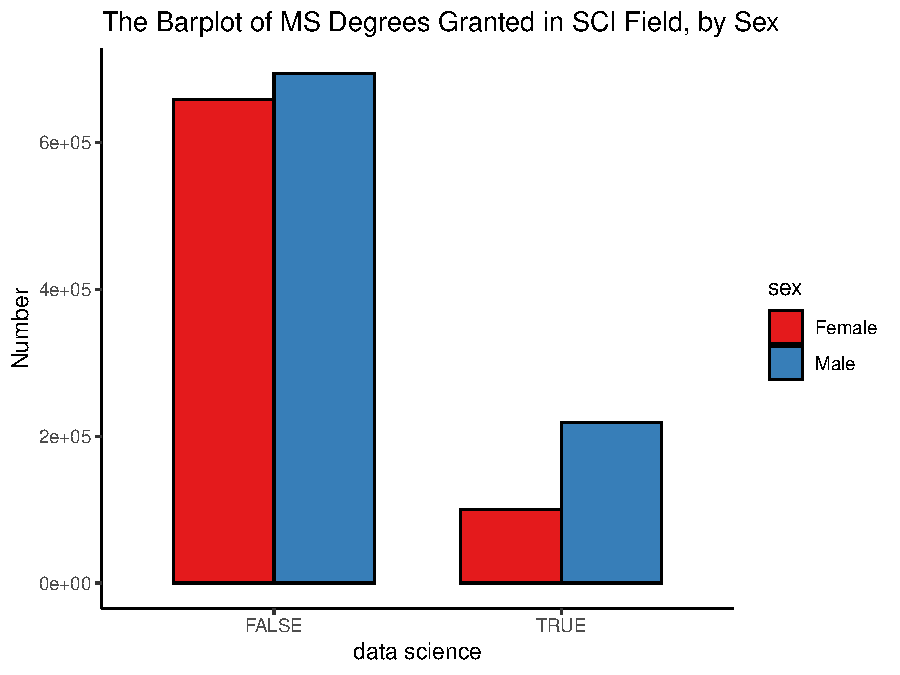
\includegraphics{hw1_sol_files/figure-latex/unnamed-chunk-12-2.pdf}

\begin{Shaded}
\begin{Highlighting}[]
\FunctionTok{ggplot}\NormalTok{(summary.ds.phd,}\FunctionTok{aes}\NormalTok{(}\AttributeTok{x=}\NormalTok{datasci,}\AttributeTok{weight=}\NormalTok{number,}\AttributeTok{fill=}\NormalTok{sex))}\SpecialCharTok{+}
  \FunctionTok{geom\_bar}\NormalTok{(}\AttributeTok{color =} \StringTok{"black"}\NormalTok{, }\AttributeTok{width =}\NormalTok{ .}\DecValTok{7}\NormalTok{,}\AttributeTok{position =} \StringTok{\textquotesingle{}dodge\textquotesingle{}}\NormalTok{)}\SpecialCharTok{+}
  \FunctionTok{theme\_classic}\NormalTok{()}\SpecialCharTok{+}
  \FunctionTok{ylab}\NormalTok{(}\StringTok{\textquotesingle{}Number\textquotesingle{}}\NormalTok{)}\SpecialCharTok{+}
  \FunctionTok{xlab}\NormalTok{(}\StringTok{\textquotesingle{}data science\textquotesingle{}}\NormalTok{)}\SpecialCharTok{+}
  \FunctionTok{scale\_fill\_brewer}\NormalTok{(}\AttributeTok{palette =} \StringTok{"Set1"}\NormalTok{)}\SpecialCharTok{+}
  \FunctionTok{labs}\NormalTok{(}\AttributeTok{title =} \StringTok{"The Barplot of PhD Degrees Granted in SCI Field, by Sex"}\NormalTok{)}
\end{Highlighting}
\end{Shaded}

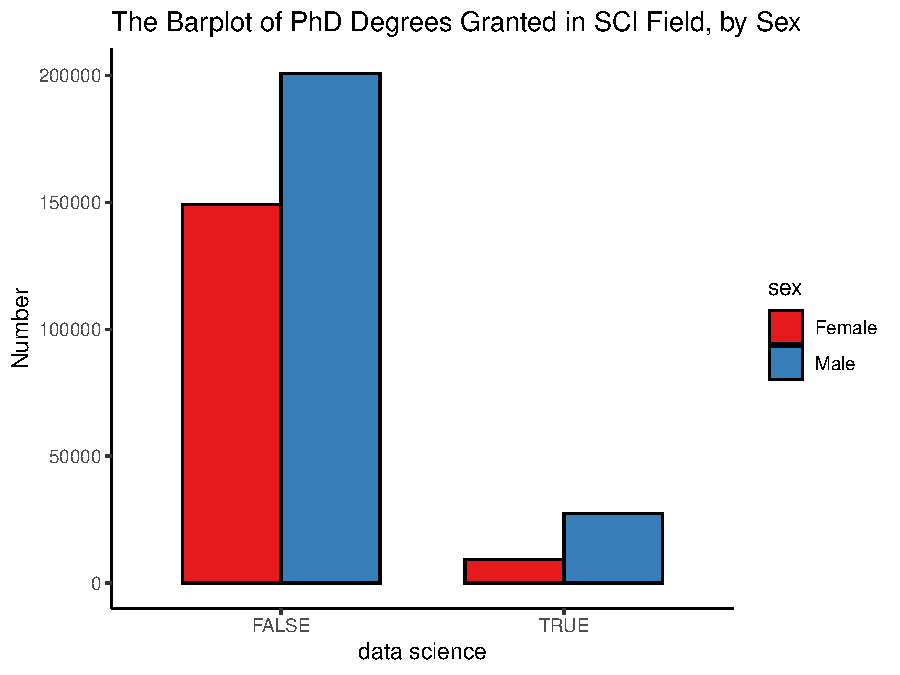
\includegraphics{hw1_sol_files/figure-latex/unnamed-chunk-12-3.pdf} \#\#
Final Report

\hypertarget{appendix}{%
\subsection{Appendix}\label{appendix}}

\hypertarget{case-study-3-major-league-baseball}{%
\section{Case Study 3: Major League
Baseball}\label{case-study-3-major-league-baseball}}

\hypertarget{data-preparation-2}{%
\subsection{Data Preparation}\label{data-preparation-2}}

\begin{Shaded}
\begin{Highlighting}[]
\FunctionTok{rm}\NormalTok{(}\AttributeTok{list =} \FunctionTok{ls}\NormalTok{())}
\NormalTok{paydata.wide }\OtherTok{=} \FunctionTok{fread}\NormalTok{(}\StringTok{"data/MLPayData\_Total.csv"}\NormalTok{, }\AttributeTok{encoding =} \StringTok{"UTF{-}8"}\NormalTok{)}
\FunctionTok{setnames}\NormalTok{(paydata.wide,}\StringTok{"Team.name.2014"}\NormalTok{,}\StringTok{"team"}\NormalTok{)}

\NormalTok{paydata.long }\OtherTok{=} \FunctionTok{fread}\NormalTok{(}\StringTok{"data/baseball.csv"}\NormalTok{, }\AttributeTok{encoding =} \StringTok{"UTF{-}8"}\NormalTok{)}

\CommentTok{\# test conversion}
\CommentTok{\# paydata.wide[,.(p1998:p2014)] \# do not try to use .() and : simultaneously. otherwise return a vector step by +1}

\CommentTok{\# pay = paydata.wide[,team,p1998:p2014] \%\textgreater{}\%}
\CommentTok{\#   pivot\_longer(cols = p1998:p2014,}
\CommentTok{\#                names\_prefix = "p",}
\CommentTok{\#                names\_to = "year",}
\CommentTok{\#                values\_to = "payroll")}
\CommentTok{\# win.num = paydata.wide[,team,X1998:X2014] \%\textgreater{}\%}
\CommentTok{\#   pivot\_longer(cols = X1998:X2014,}
\CommentTok{\#                names\_prefix = "X",}
\CommentTok{\#                names\_to = "year",}
\CommentTok{\#                values\_to = "win.num")}
\CommentTok{\# win.per = paydata.wide[,team,X1998.pct:X2014.pct] \%\textgreater{}\%}
\CommentTok{\#   pivot\_longer(cols = X1998.pct:X2014.pct,}
\CommentTok{\#                names\_prefix = "X",}
\CommentTok{\#                names\_to = "year",}
\CommentTok{\#                values\_to = "win.pct") \%\textgreater{}\%}
\CommentTok{\#   mutate(year = substr(year,1,4))}
\CommentTok{\# test.long = pay \%\textgreater{}\%}
\CommentTok{\#   right\_join(win.num, by = c("year","team")) \%\textgreater{}\%}
\CommentTok{\#   right\_join(win.per, by = c("year","team"))}

\CommentTok{\# create increments}
\NormalTok{paydata.long[}\FunctionTok{order}\NormalTok{(team,year),log.pay }\SpecialCharTok{:}\ErrorTok{=} \FunctionTok{log}\NormalTok{(payroll)]}
\NormalTok{paydata.long[,pay.diff }\SpecialCharTok{:}\ErrorTok{=} \FunctionTok{c}\NormalTok{(}\ConstantTok{NA}\NormalTok{,}\FunctionTok{diff}\NormalTok{(payroll)),by }\OtherTok{=}\NormalTok{ team]}
\NormalTok{paydata.long[,log.pay.diff }\SpecialCharTok{:}\ErrorTok{=} \FunctionTok{c}\NormalTok{(}\ConstantTok{NA}\NormalTok{,}\FunctionTok{diff}\NormalTok{(log.pay)),by }\OtherTok{=}\NormalTok{ team]}
\NormalTok{paydata.new }\OtherTok{=}\NormalTok{ paydata.long[,.(team,year,}\AttributeTok{diff\_log=}\NormalTok{log.pay.diff,win\_pct)]}
\end{Highlighting}
\end{Shaded}

The log difference is more appropriate in this setup because it measures
the proportional (relative) change in the payroll. The base payrolls in
all teams are not the same, so a same increase in absolute amount may
incentivize players differently in different teams; the incentive may be
bigger in teams with a smaller payroll, but smaller in teams with a
larger payroll. The relative changes measured by the difference of
logarithm of payroll can alleviate this problem.

\hypertarget{exploratory-questions}{%
\subsection{Exploratory Questions}\label{exploratory-questions}}

\begin{Shaded}
\begin{Highlighting}[]
\NormalTok{increase.data }\OtherTok{=}\NormalTok{ paydata.new[year }\SpecialCharTok{\%in\%} \DecValTok{2010}\SpecialCharTok{:}\DecValTok{2014}\NormalTok{,.(}
  \AttributeTok{pay.increase =} \FunctionTok{sum}\NormalTok{(diff\_log[}\SpecialCharTok{{-}}\DecValTok{1}\NormalTok{]), }\CommentTok{\# from 2010 to 2014, increase in log(payroll)}
  \AttributeTok{win.pct.increase =}\NormalTok{ win\_pct[}\FunctionTok{length}\NormalTok{(win\_pct)]}\SpecialCharTok{{-}}\NormalTok{win\_pct[}\DecValTok{1}\NormalTok{] }
\NormalTok{), by }\OtherTok{=}\NormalTok{ team]}
\NormalTok{increase.data }\SpecialCharTok{\%\textgreater{}\%}
  \FunctionTok{filter}\NormalTok{(}\FunctionTok{rank}\NormalTok{(}\SpecialCharTok{{-}}\NormalTok{pay.increase)}\SpecialCharTok{\textless{}}\DecValTok{6}\NormalTok{) }\SpecialCharTok{\%\textgreater{}\%}
  \FunctionTok{select}\NormalTok{(team) }\CommentTok{\# top 5 teams in payroll increase}
\end{Highlighting}
\end{Shaded}

\begin{verbatim}
##                    team
## 1:  Los Angeles Dodgers
## 2:   Pittsburgh Pirates
## 3:     San Diego Padres
## 4:        Texas Rangers
## 5: Washington Nationals
\end{verbatim}

\begin{Shaded}
\begin{Highlighting}[]
\NormalTok{increase.data }\SpecialCharTok{\%\textgreater{}\%}
  \FunctionTok{filter}\NormalTok{(}\FunctionTok{rank}\NormalTok{(}\SpecialCharTok{{-}}\NormalTok{win.pct.increase)}\SpecialCharTok{\textless{}}\DecValTok{6}\NormalTok{) }\SpecialCharTok{\%\textgreater{}\%}
  \FunctionTok{select}\NormalTok{(team) }\CommentTok{\# top 5 teams in winning percentage increase}
\end{Highlighting}
\end{Shaded}

\begin{verbatim}
##                    team
## 1:    Baltimore Orioles
## 2:   Kansas City Royals
## 3:   Pittsburgh Pirates
## 4:     Seattle Mariners
## 5: Washington Nationals
\end{verbatim}

\hypertarget{prediction}{%
\subsection{prediction}\label{prediction}}

\begin{Shaded}
\begin{Highlighting}[]
\CommentTok{\# 2010{-}2014}
\FunctionTok{ggplot}\NormalTok{(increase.data,}\FunctionTok{aes}\NormalTok{(}\AttributeTok{x=}\NormalTok{pay.increase,}\AttributeTok{y=}\NormalTok{win.pct.increase))}\SpecialCharTok{+}
  \FunctionTok{geom\_point}\NormalTok{(}\AttributeTok{color=}\StringTok{"blue"}\NormalTok{,}\AttributeTok{size=}\FloatTok{1.5}\NormalTok{)}\SpecialCharTok{+}
  \FunctionTok{geom\_smooth}\NormalTok{(}\AttributeTok{method =} \StringTok{"lm"}\NormalTok{,}\AttributeTok{formula =}\NormalTok{ y}\SpecialCharTok{\textasciitilde{}}\NormalTok{x, }\AttributeTok{color=}\StringTok{"red"}\NormalTok{)}\SpecialCharTok{+}
  \FunctionTok{geom\_text\_repel}\NormalTok{(}\FunctionTok{aes}\NormalTok{(}\AttributeTok{label =}\NormalTok{ team))}\SpecialCharTok{+}
  \FunctionTok{xlab}\NormalTok{(}\StringTok{"increase in payroll, 2010{-}2014"}\NormalTok{)}\SpecialCharTok{+}
  \FunctionTok{ylab}\NormalTok{(}\StringTok{"increase in winning percentage, 2010{-}2014"}\NormalTok{)}\SpecialCharTok{+}
  \FunctionTok{theme\_bw}\NormalTok{()}\SpecialCharTok{+}
  \FunctionTok{labs}\NormalTok{(}\StringTok{"Relationship between Payroll Increase and Performance Increase, 2010{-}2014"}\NormalTok{)}
\end{Highlighting}
\end{Shaded}

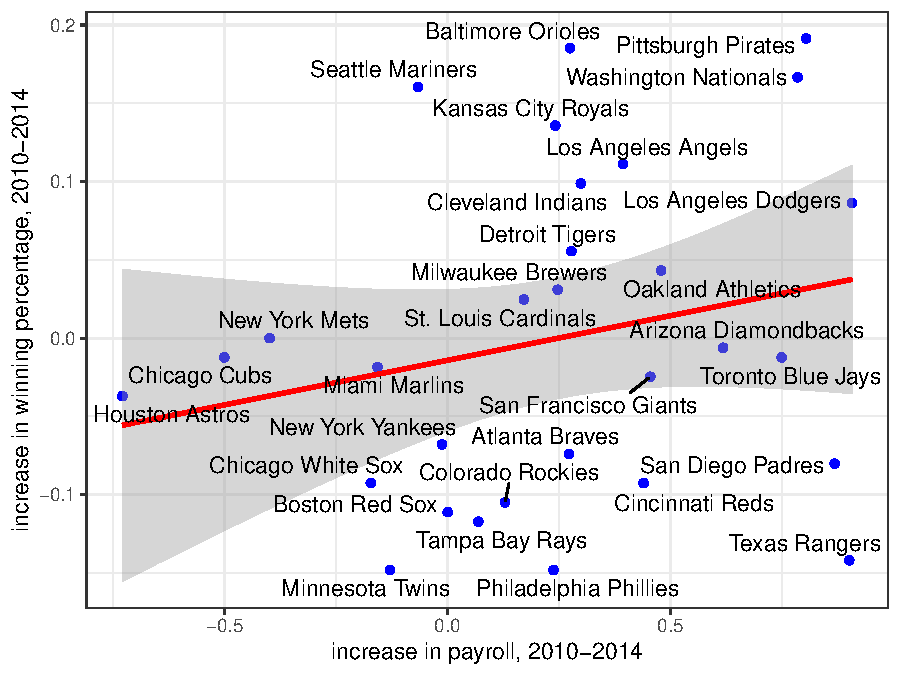
\includegraphics{hw1_sol_files/figure-latex/unnamed-chunk-16-1.pdf}

\begin{Shaded}
\begin{Highlighting}[]
\CommentTok{\# all years, year{-}on{-}year basis}
\NormalTok{paydata.long[,diff\_win\_pct }\SpecialCharTok{:}\ErrorTok{=} \FunctionTok{c}\NormalTok{(}\ConstantTok{NA}\NormalTok{,}\FunctionTok{diff}\NormalTok{(win\_pct)), by }\OtherTok{=}\NormalTok{ team]}

\FunctionTok{ggplot}\NormalTok{(paydata.long,}\FunctionTok{aes}\NormalTok{(}\AttributeTok{x=}\NormalTok{log.pay.diff,}\AttributeTok{y=}\NormalTok{diff\_win\_pct))}\SpecialCharTok{+}
  \FunctionTok{geom\_point}\NormalTok{(}\AttributeTok{color=}\StringTok{"blue"}\NormalTok{,}\AttributeTok{size=}\FloatTok{1.5}\NormalTok{)}\SpecialCharTok{+}
  \FunctionTok{geom\_smooth}\NormalTok{(}\AttributeTok{method =} \StringTok{"lm"}\NormalTok{, }\AttributeTok{formula =}\NormalTok{ y}\SpecialCharTok{\textasciitilde{}}\NormalTok{x, }\AttributeTok{color=}\StringTok{"red"}\NormalTok{)}\SpecialCharTok{+}
  \FunctionTok{xlab}\NormalTok{(}\StringTok{"increase in payroll, year on year"}\NormalTok{)}\SpecialCharTok{+}
  \FunctionTok{ylab}\NormalTok{(}\StringTok{"increase in winning percentage, year on year"}\NormalTok{)}\SpecialCharTok{+}
  \FunctionTok{theme\_bw}\NormalTok{()}\SpecialCharTok{+}
  \FunctionTok{labs}\NormalTok{(}\StringTok{"Relationship between Payroll Increase and Performance Increase, All Years"}\NormalTok{)}
\end{Highlighting}
\end{Shaded}

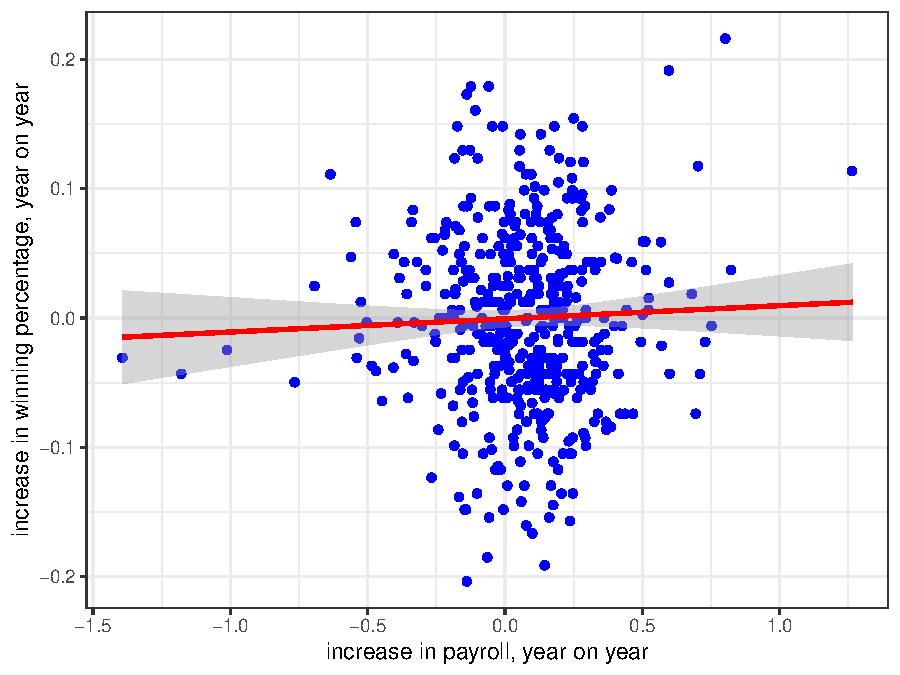
\includegraphics{hw1_sol_files/figure-latex/unnamed-chunk-16-2.pdf}

\begin{Shaded}
\begin{Highlighting}[]
\FunctionTok{summary}\NormalTok{(}\FunctionTok{lm}\NormalTok{(diff\_win\_pct}\SpecialCharTok{\textasciitilde{}}\NormalTok{log.pay.diff,}\AttributeTok{data =}\NormalTok{ paydata.long)) }\CommentTok{\# not significant}
\end{Highlighting}
\end{Shaded}

\begin{verbatim}
## 
## Call:
## lm(formula = diff_win_pct ~ log.pay.diff, data = paydata.long)
## 
## Residuals:
##       Min        1Q    Median        3Q       Max 
## -0.201605 -0.044979 -0.001237  0.043731  0.208554 
## 
## Coefficients:
##                Estimate Std. Error t value Pr(>|t|)
## (Intercept)  -0.0006855  0.0032666  -0.210    0.834
## log.pay.diff  0.0102008  0.0123781   0.824    0.410
## 
## Residual standard error: 0.06919 on 478 degrees of freedom
##   (30 observations deleted due to missingness)
## Multiple R-squared:  0.001419,   Adjusted R-squared:  -0.0006703 
## F-statistic: 0.6791 on 1 and 478 DF,  p-value: 0.4103
\end{verbatim}

\begin{Shaded}
\begin{Highlighting}[]
\CommentTok{\# how about next year?}
\NormalTok{paydata.long[,diff\_win\_pct\_next }\SpecialCharTok{:}\ErrorTok{=} \FunctionTok{c}\NormalTok{(}\FunctionTok{diff}\NormalTok{(win\_pct),}\ConstantTok{NA}\NormalTok{), by }\OtherTok{=}\NormalTok{ team]}

\FunctionTok{ggplot}\NormalTok{(paydata.long,}\FunctionTok{aes}\NormalTok{(}\AttributeTok{x=}\NormalTok{log.pay.diff,}\AttributeTok{y=}\NormalTok{diff\_win\_pct\_next))}\SpecialCharTok{+}
  \FunctionTok{geom\_point}\NormalTok{(}\AttributeTok{color=}\StringTok{"blue"}\NormalTok{,}\AttributeTok{size=}\FloatTok{1.5}\NormalTok{)}\SpecialCharTok{+}
  \FunctionTok{geom\_smooth}\NormalTok{(}\AttributeTok{method =} \StringTok{"lm"}\NormalTok{, }\AttributeTok{formula =}\NormalTok{ y}\SpecialCharTok{\textasciitilde{}}\NormalTok{x, }\AttributeTok{color=}\StringTok{"red"}\NormalTok{)}\SpecialCharTok{+}
  \FunctionTok{xlab}\NormalTok{(}\StringTok{"increase in payroll, year on year"}\NormalTok{)}\SpecialCharTok{+}
  \FunctionTok{ylab}\NormalTok{(}\StringTok{"increase in winning percentage next year, year on year"}\NormalTok{)}\SpecialCharTok{+}
  \FunctionTok{theme\_bw}\NormalTok{()}\SpecialCharTok{+}
  \FunctionTok{labs}\NormalTok{(}\StringTok{"Relationship between Payroll Increase and Performance Increase Next Year, All Years"}\NormalTok{)}
\end{Highlighting}
\end{Shaded}

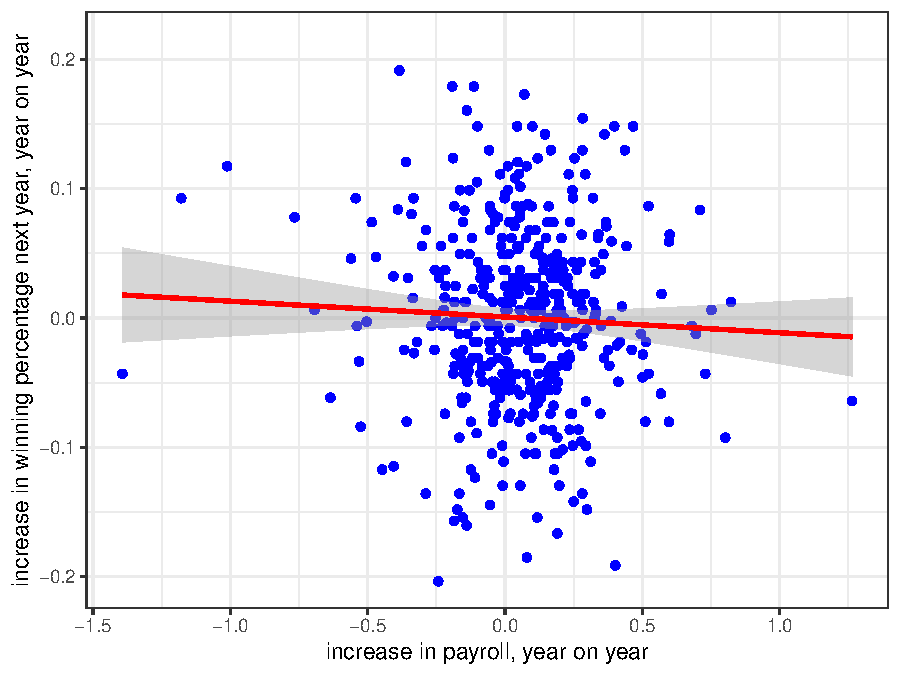
\includegraphics{hw1_sol_files/figure-latex/unnamed-chunk-16-3.pdf}

\begin{Shaded}
\begin{Highlighting}[]
\FunctionTok{summary}\NormalTok{(}\FunctionTok{lm}\NormalTok{(diff\_win\_pct\_next}\SpecialCharTok{\textasciitilde{}}\NormalTok{log.pay.diff,}\AttributeTok{data =}\NormalTok{ paydata.long)) }\CommentTok{\# negative and not significant}
\end{Highlighting}
\end{Shaded}

\begin{verbatim}
## 
## Call:
## lm(formula = diff_win_pct_next ~ log.pay.diff, data = paydata.long)
## 
## Residuals:
##       Min        1Q    Median        3Q       Max 
## -0.207438 -0.045105 -0.000575  0.045353  0.185903 
## 
## Coefficients:
##                Estimate Std. Error t value Pr(>|t|)
## (Intercept)   0.0007709  0.0033460   0.230    0.818
## log.pay.diff -0.0121974  0.0125591  -0.971    0.332
## 
## Residual standard error: 0.069 on 448 degrees of freedom
##   (60 observations deleted due to missingness)
## Multiple R-squared:  0.002101,   Adjusted R-squared:  -0.0001265 
## F-statistic: 0.9432 on 1 and 448 DF,  p-value: 0.332
\end{verbatim}

\begin{Shaded}
\begin{Highlighting}[]
\CommentTok{\# payroll to winning percentage}
\FunctionTok{ggplot}\NormalTok{(paydata.long,}\FunctionTok{aes}\NormalTok{(}\AttributeTok{x=}\NormalTok{log.pay,}\AttributeTok{y=}\NormalTok{win\_pct))}\SpecialCharTok{+}
  \FunctionTok{geom\_point}\NormalTok{(}\AttributeTok{color=}\StringTok{"blue"}\NormalTok{,}\AttributeTok{size=}\FloatTok{1.5}\NormalTok{)}\SpecialCharTok{+}
  \FunctionTok{geom\_smooth}\NormalTok{(}\AttributeTok{method =} \StringTok{"lm"}\NormalTok{, }\AttributeTok{formula =}\NormalTok{ y}\SpecialCharTok{\textasciitilde{}}\NormalTok{x, }\AttributeTok{color=}\StringTok{"red"}\NormalTok{)}\SpecialCharTok{+}
  \FunctionTok{xlab}\NormalTok{(}\StringTok{"log payroll"}\NormalTok{)}\SpecialCharTok{+}
  \FunctionTok{ylab}\NormalTok{(}\StringTok{"winning percentage"}\NormalTok{)}\SpecialCharTok{+}
  \FunctionTok{theme\_bw}\NormalTok{()}\SpecialCharTok{+}
  \FunctionTok{labs}\NormalTok{(}\StringTok{"Relationship between Payroll and Performance, All Years"}\NormalTok{)}
\end{Highlighting}
\end{Shaded}

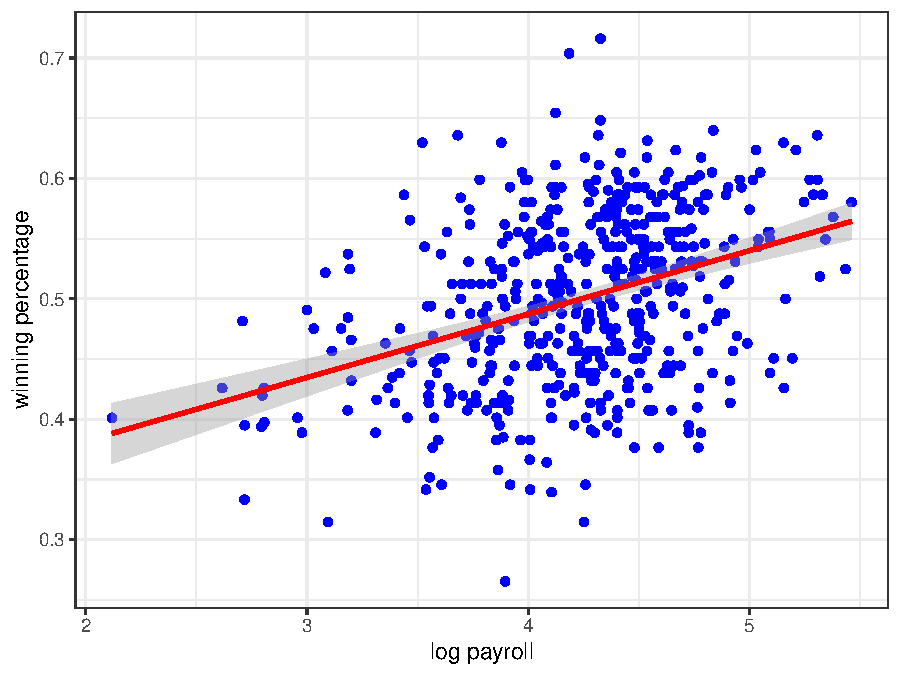
\includegraphics{hw1_sol_files/figure-latex/unnamed-chunk-17-1.pdf}

\begin{Shaded}
\begin{Highlighting}[]
\FunctionTok{summary}\NormalTok{(}\FunctionTok{lm}\NormalTok{(win\_pct}\SpecialCharTok{\textasciitilde{}}\NormalTok{log.pay,}\AttributeTok{data =}\NormalTok{ paydata.long)) }\CommentTok{\# good prediction}
\end{Highlighting}
\end{Shaded}

\begin{verbatim}
## 
## Call:
## lm(formula = win_pct ~ log.pay, data = paydata.long)
## 
## Residuals:
##      Min       1Q   Median       3Q      Max 
## -0.21640 -0.04691  0.00447  0.05019  0.21151 
## 
## Coefficients:
##             Estimate Std. Error t value Pr(>|t|)    
## (Intercept) 0.276629   0.024943  11.090   <2e-16 ***
## log.pay     0.052682   0.005842   9.018   <2e-16 ***
## ---
## Signif. codes:  0 '***' 0.001 '**' 0.01 '*' 0.05 '.' 0.1 ' ' 1
## 
## Residual standard error: 0.06678 on 508 degrees of freedom
## Multiple R-squared:  0.138,  Adjusted R-squared:  0.1363 
## F-statistic: 81.32 on 1 and 508 DF,  p-value: < 2.2e-16
\end{verbatim}

\begin{Shaded}
\begin{Highlighting}[]
\CommentTok{\# payroll to increase in winning percentage next year}
\FunctionTok{ggplot}\NormalTok{(paydata.long,}\FunctionTok{aes}\NormalTok{(}\AttributeTok{x=}\NormalTok{log.pay,}\AttributeTok{y=}\NormalTok{diff\_win\_pct\_next))}\SpecialCharTok{+}
  \FunctionTok{geom\_point}\NormalTok{(}\AttributeTok{color=}\StringTok{"blue"}\NormalTok{,}\AttributeTok{size=}\FloatTok{1.5}\NormalTok{)}\SpecialCharTok{+}
  \FunctionTok{geom\_smooth}\NormalTok{(}\AttributeTok{method =} \StringTok{"lm"}\NormalTok{, }\AttributeTok{formula =}\NormalTok{ y}\SpecialCharTok{\textasciitilde{}}\NormalTok{x, }\AttributeTok{color=}\StringTok{"red"}\NormalTok{)}\SpecialCharTok{+}
  \FunctionTok{xlab}\NormalTok{(}\StringTok{"log payroll"}\NormalTok{)}\SpecialCharTok{+}
  \FunctionTok{ylab}\NormalTok{(}\StringTok{"increase in winning percentage next year, year on year"}\NormalTok{)}\SpecialCharTok{+}
  \FunctionTok{theme\_bw}\NormalTok{()}\SpecialCharTok{+}
  \FunctionTok{labs}\NormalTok{(}\StringTok{"Relationship between Payroll and Performance Increase Next Year, All Years"}\NormalTok{)}
\end{Highlighting}
\end{Shaded}

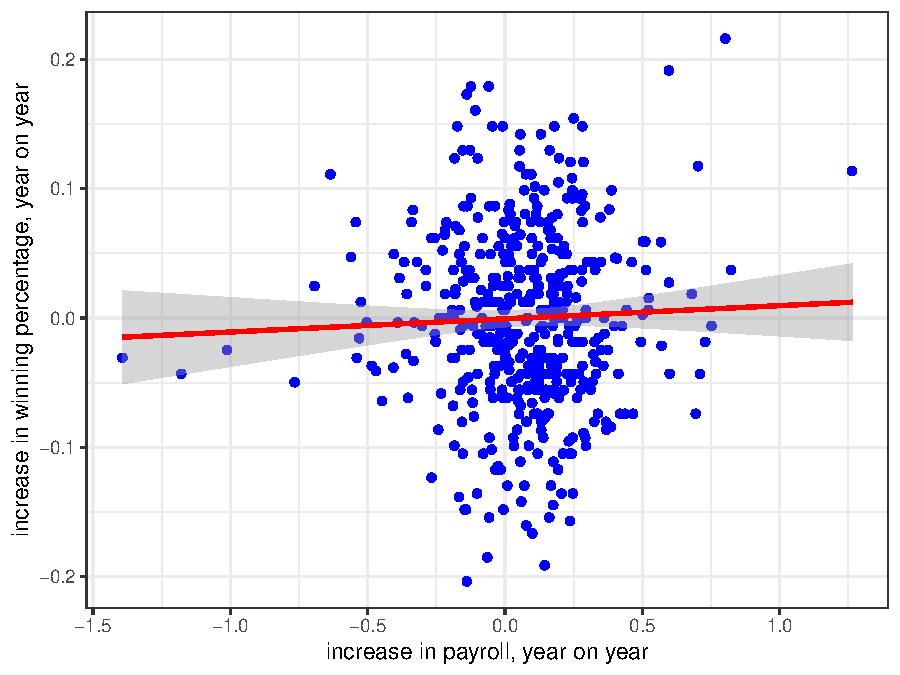
\includegraphics{hw1_sol_files/figure-latex/unnamed-chunk-17-2.pdf}

\begin{Shaded}
\begin{Highlighting}[]
\FunctionTok{summary}\NormalTok{(}\FunctionTok{lm}\NormalTok{(diff\_win\_pct\_next}\SpecialCharTok{\textasciitilde{}}\NormalTok{log.pay,}\AttributeTok{data =}\NormalTok{ paydata.long)) }\CommentTok{\# not bad prediction? can be spurred}
\end{Highlighting}
\end{Shaded}

\begin{verbatim}
## 
## Call:
## lm(formula = diff_win_pct_next ~ log.pay, data = paydata.long)
## 
## Residuals:
##       Min        1Q    Median        3Q       Max 
## -0.200438 -0.046946 -0.000896  0.044609  0.202100 
## 
## Coefficients:
##              Estimate Std. Error t value Pr(>|t|)   
## (Intercept)  0.077443   0.026526   2.919  0.00367 **
## log.pay     -0.018385   0.006253  -2.940  0.00344 **
## ---
## Signif. codes:  0 '***' 0.001 '**' 0.01 '*' 0.05 '.' 0.1 ' ' 1
## 
## Residual standard error: 0.06862 on 478 degrees of freedom
##   (30 observations deleted due to missingness)
## Multiple R-squared:  0.01776,    Adjusted R-squared:  0.01571 
## F-statistic: 8.643 on 1 and 478 DF,  p-value: 0.003442
\end{verbatim}

\begin{Shaded}
\begin{Highlighting}[]
\CommentTok{\# pay roll to increase in winning percentage current year}
\FunctionTok{ggplot}\NormalTok{(paydata.long,}\FunctionTok{aes}\NormalTok{(}\AttributeTok{x=}\NormalTok{log.pay,}\AttributeTok{y=}\NormalTok{diff\_win\_pct))}\SpecialCharTok{+}
  \FunctionTok{geom\_point}\NormalTok{(}\AttributeTok{color=}\StringTok{"blue"}\NormalTok{,}\AttributeTok{size=}\FloatTok{1.5}\NormalTok{)}\SpecialCharTok{+}
  \FunctionTok{geom\_smooth}\NormalTok{(}\AttributeTok{method =} \StringTok{"lm"}\NormalTok{, }\AttributeTok{formula =}\NormalTok{ y}\SpecialCharTok{\textasciitilde{}}\NormalTok{x, }\AttributeTok{color=}\StringTok{"red"}\NormalTok{)}\SpecialCharTok{+}
  \FunctionTok{xlab}\NormalTok{(}\StringTok{"log payroll"}\NormalTok{)}\SpecialCharTok{+}
  \FunctionTok{ylab}\NormalTok{(}\StringTok{"increase in winning percentage, year on year"}\NormalTok{)}\SpecialCharTok{+}
  \FunctionTok{theme\_bw}\NormalTok{()}\SpecialCharTok{+}
  \FunctionTok{labs}\NormalTok{(}\StringTok{"Relationship between Payroll and Performance Increase Next Year, All Years"}\NormalTok{)}
\end{Highlighting}
\end{Shaded}

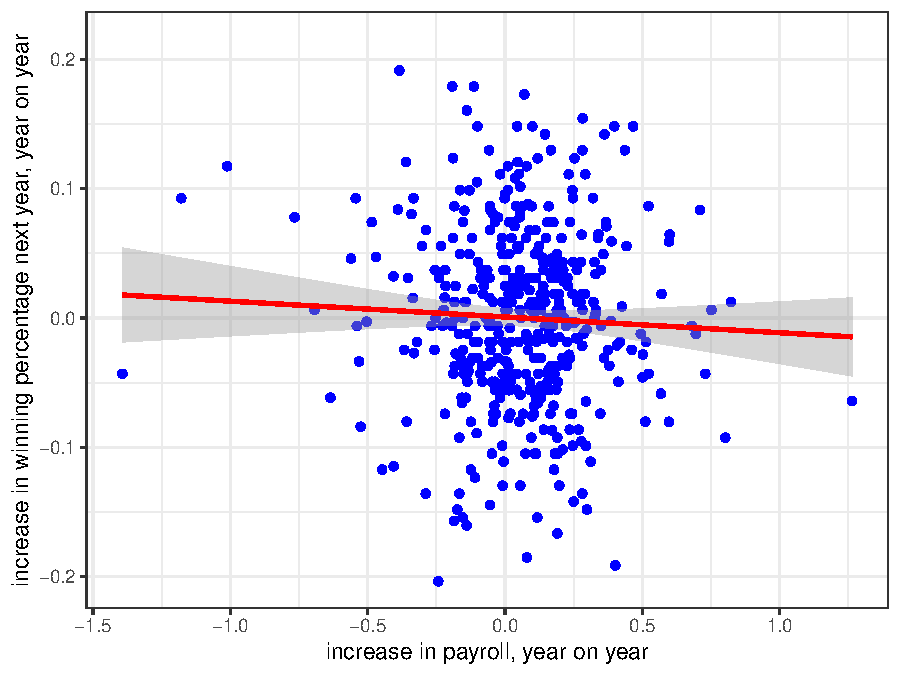
\includegraphics{hw1_sol_files/figure-latex/unnamed-chunk-17-3.pdf}

\begin{Shaded}
\begin{Highlighting}[]
\FunctionTok{summary}\NormalTok{(}\FunctionTok{lm}\NormalTok{(diff\_win\_pct}\SpecialCharTok{\textasciitilde{}}\NormalTok{log.pay,}\AttributeTok{data =}\NormalTok{ paydata.long)) }\CommentTok{\# not bad prediction? can be spurred}
\end{Highlighting}
\end{Shaded}

\begin{verbatim}
## 
## Call:
## lm(formula = diff_win_pct ~ log.pay, data = paydata.long)
## 
## Residuals:
##       Min        1Q    Median        3Q       Max 
## -0.204195 -0.046024 -0.001478  0.044662  0.215630 
## 
## Coefficients:
##              Estimate Std. Error t value Pr(>|t|)   
## (Intercept)  0.074104   0.028295   2.619  0.00910 **
## log.pay     -0.017315   0.006571  -2.635  0.00868 **
## ---
## Signif. codes:  0 '***' 0.001 '**' 0.01 '*' 0.05 '.' 0.1 ' ' 1
## 
## Residual standard error: 0.06874 on 478 degrees of freedom
##   (30 observations deleted due to missingness)
## Multiple R-squared:  0.01432,    Adjusted R-squared:  0.01226 
## F-statistic: 6.944 on 1 and 478 DF,  p-value: 0.008683
\end{verbatim}

\begin{Shaded}
\begin{Highlighting}[]
\CommentTok{\# The last two prediction power should be taken cautiously. It may stem from some rising small teams}
\end{Highlighting}
\end{Shaded}

Overall, current payroll predicts current performance well. As for
changes in performance, there is weak evidence that increase in current
performance is positively correlated to increase in payroll, but still
not very predictive. It is surprising that the increase in performance,
no matter current or future, is negatively correlated with the current
payroll, to some degree. However, we should be cautious about this
conclusion as it may be mainly driven by some rising small teams.

One more thing to note is that correlation does not mean causality.

\begin{Shaded}
\begin{Highlighting}[]
\FunctionTok{save.image}\NormalTok{(}\StringTok{"hw1.RData"}\NormalTok{)}
\end{Highlighting}
\end{Shaded}


\end{document}
